\chapter{Eigensimilarity based Framework for Detection and Identification of Network Attacks}
\label{ch:2_mos_eig_sim}

According to \cite{Hevesi2019}, at times, organizations relate their security measures to confidentiality and integrity, ignoring availability. However, according to \cite{BISSELL2019}, the global average annual cost of DoS attack was US\$1.7 million in 2018.

The Denial of Service (DoS) attack attempts to deny access to system or network resources, attacking the availability of the service, by means of flooding techniques for consuming the available resources, or by means of subtle approaches which send small amount of data that can cause failure and unavailability of the system. In 2017 the top motivation behind DDoS attacks was criminals demonstrating attack capabilities, with gaming and criminal extortion attempts in second and third place, respectively \cite{cisco2019}.

With application layer Distributed Denial of Service (DDoS) attacks continuing to rise, vendors have begun adding DDoS mitigation features into solutions that protect web applications \cite{Hevesi2019}. The leading solutions for monitoring and mitigation of DDoS attacks in application layer start with behavioral analytics and supplement with signature-based detection for known malicious application attacks \cite{Hevesi2019}.

Probe attacks aim to scan the networks to identify running services, open ports, running services and vulnerabilities that can be exploited. A probe attack is considered the first step in an attack to compromise a host or network. Although no specific damage is caused by these attacks, they are considered serious threats by \cite{ahmed2016survey} and \cite{moustafa2019holistic}. Note that we refer to port scan as an attack, according to \cite{ahmed2016survey}.

Anomaly-based systems for network attack detection focus on finding exceptional, suspicious or rare observations in network traffic that do not conform to the expected normal behavior \cite{bhuyan2014network}. It is possible to adopt unsupervised or semi-supervised approaches for network anomaly detection, by means of behavioral analysis, where known anomalies for training models are not necessary \cite{moustafa2019holistic}. 

Recently, signal processing schemes have been applied for network anomaly detection in computer networks by means of unsupervised approaches, showing advances in network traffic analysis \cite{Zonglin2009}, in network attack detection \cite{callegari2011novel}, and in network anomaly detection based on network flows \cite{Lu2009}.

Considering that a subspace learned by eigenvalue decomposition can highlight anomalies for network attack detection by means of model order selection (MOS), and that the comparison between the principal eigenvectors can reveal anomalies when comparing legitimate and anomalous observations. In this chapter we propose the Eigensimilarity, which is an approach based on signal processing concepts applied to detection of malicious traffic in computer networks, with focus on DoS and portscan attacks. 

The Eigensimilarity is based on eigenvalue analysis, model order selection (MOS) and similarity analysis between the principal eigenvectors. In contrast to \cite{david2011blind, da2012improved, tenorio2013greatest}, MOS and eigenvalue analysis are applied to detect time frames under attack, and the analysis of similarity between the principal eigenvectors are used for precise identification of the time and ports under attack. In addition, we evaluate the accuracy and performance of the proposed framework applied to an experimental scenario and to the DARPA 1998 data set \citep{osanaiye2016distributed}, which is a well-known network traffic data set. 

The performed experiments show that synflood, fraggle and port scan attacks can be accurately detected and with great detail in an automatic and blind fashion, i.e. in an unsupervised approach that does not require data for training, applying signal processing concepts for traffic modeling and through approaches based on MOS and principal eigenvector similarity analysis. The main contributions of the proposed framework are the capability to blindly detect time frames under network attack via MOS and eigen analysis, and the detailed identification of the network attack via principal eigenvector similarity analysis.

This chapter is organized as follows. In Section \ref{sec:2_relatedworks} the related works are discussed. We present the data model and the evaluated data sets in Section \ref{sec:2_datamodel} and the proposed framework for blind and automatic detection of flood and probe attacks is described in Section \ref{sec:2_prop_getv}. The discussion of the experimental validation and results are presented in Section \ref{sec:2_experimentalresults}, while the discussion of the computational complexity and evaluation of the required processing time for tested scenarios are presented in Section \ref{sec:2_Complexity}. In Section \ref{sec:2_conclusionandfutureworks} we draw the conclusions and the suggestions for future work.


\section{Related Works}
\label{sec:2_relatedworks}

Several methods have been proposed for the identification and characterization of malicious activity in computer networks. Classical methods typically employ data mining \cite{he2008applying,ghourabi2010data,osanaiye2016distributed} and regular file analysis \cite{raynal2004honeypot} to detect patterns that indicate the presence of specific attacks in network traffic.

Data mining is often used to describe the process of extracting useful information from large databases. Multiple methods of data mining are used in \cite{he2008applying,osanaiye2016distributed} to analyze data flow in a network with the aim of identifying characteristics of malicious traffic in large scale environments. Researchers have applied data mining techniques in log analysis \cite{ghourabi2010data} to improve intrusion detection performance. However, data mining techniques used so far in network analysis require prior collection of large data sets, which is a limitation of several schemes for online analysis \cite{he2008applying}.

Regular file analysis \cite{raynal2004honeypot} consists of traffic analysis for detecting known patterns that indicate the presence of attacks, applying statistical analysis to the study of collected traffic. An essential feature of this method is that it depends on prior knowledge of the details of the attacks to be identified, and also depends on previous log collection for traffic analysis and false positives reduction.

Principal Component Analysis (PCA) is a statistical technique commonly used for dimensionality reduction. It uses an orthogonal transformation to convert a set of correlated variables into a new subspace of linearly uncorrelated variables, by means of eigenvalue value decomposition, where the first principal components have the largest variance. PCA has been used in attack detection \cite{almotairi2009technique}, considering that this technique is very sensitive to outliers and adopted for classification problems. However, PCA requires human intervention in order to identify abnormalities based on the eigenvalues profiles, if used without complementary techniques.

Callegari \emph{et al.} \cite{callegari2011novel} proposed a PCA-based method for identifying the traffic flows responsible for an anomaly detected at the aggregate level and evaluated their proposal through a data set with synthetic anomalies added in the data. However, Callegari \emph{et al.} \cite{callegari2011novel} focus on flood attack detection, not addressing probe attack detection, and their approach relies on visual analysis. 

Lee \emph{et al.} \cite{Lee2013} presented the OverSampling PCA (osPCA), which allows one to determine the anomaly of the target instance according to the variation of the resulting dominant eigenvector obtained by similarity analysis and over sampling. In contrast to Lee \emph{et al.} \cite{Lee2013}, the Eigensimilarity applies MOS for detection of time frames under attack and similarity analysis to extract details for detection of time and ports under attack. Additionally, Lee \emph{et al.} \cite{Lee2013} only evaluate their proposed scheme for covariance analysis, while we adopt an analysis based on sample covariance of zero mean variables and sample covariance of zero mean and unitary standard deviation variables, for flood and probe attacks, respectively. 

Signal processing techniques have been successfully applied to network anomaly detection \cite{Lu2009}. Lu and Ghorbani \cite{Lu2009} proposed a network anomaly detection model based on network flow, wavelet approximation, and system identification theory. However, their work requires a training method to produce a prediction model for normal daily traffic and presents limitations on identification of behaviors without significant outliers, such as port scan attacks. Zonglin \emph{et al.} \cite{Zonglin2009} proposed a signal processing method to detect traffic anomaly with correlation analysis, where the correlation between traffic signals and the predicted traffic signals are used to reveal anomalies. Zonglin \emph{et al.} \cite{Zonglin2009} evaluated the correlation analysis for anomaly detection, but the work is not applied for probe attack detection and does not evaluate results for attack detection on DARPA data set.

The data collected from honeypot systems, such as captured traffic and operating system logs, can be analyzed to obtain information about attack techniques, general trends of threats and exploits \cite{david2011parallel}. Blind automatic detection of malicious traffic techniques have been developed for honeypots in \cite{david2011blind, da2012improved}. However, traffic on honeypot is simpler than real network traffic, because there are no running legitimate applications, i.e. background traffic, due to the fact that honeypots emulate behavior of a host within a network to deceive and lure attackers \cite{zakaria2012review}. Since honeypots do not generate legitimate traffic, the amount of data captured in honeypots is significantly lower in comparison to a Network Intrusion Detection System (NIDS), which captures and analyzes the largest possible amount of network traffic \cite{david2011blind}. 

MOS for blind identification of malicious activities in honeypots was proposed by us in \cite{david2011blind}, which evaluated criteria for selecting the model order, through simulations and comparing the order of the resulting model with the true model order.

The proposed framework does not require either a significant amount of logs to detect attacks, nor prior data collection, in order to make comparisons and evaluate the existence of malicious traffic. The proposed solution is automatic and blind for detection of time frames under probe and flood attacks through MOS and eigen analysis. Moreover, we apply principal eigenvector similarity analysis to identify details of time and ports under network attacks.

Ahmed \emph{et al.} \cite{ahmed2016survey} highlight a observed lack of publicly available labeled data set for network anomaly detection, and discuss recent research related to overcome the issues of publicly available network intrusion evaluation data sets, including a list of current data sets and an evaluation of attack types and available labels. According to \cite{ahmed2016survey}, the available data sets present limitations on availability of labeled traffic for classification of background, legitimate and malicious traffic. The data imbalance between legitimate and malicious traffic is a important concern for real world problems of network attack, but the principal data sets usually adopt a balanced distribution between legitimate and malicious traffic, what make the attack detection more feasible for general classifiers and machine learning algorithms than for anomaly detection algorithms. Moreover, according to Ahmed \emph{et al.} \cite{ahmed2016survey}, the most adopted data set are not up-to-date with current or novel attacks, tools, operational systems and network topology.

Several approaches for network attack detection uses the KDD 99 \cite{ji2016multi, ahmed2016survey, osanaiye2016distributed, bhuyan2014network} data sets for accuracy and performance evaluation, due to their availability and labeled attacks. Even though the KDD 99 data set are criticized by for the generation procedure and the risk of over-estimations of anomaly detection due to data redundancy, it still represents one of the few publicly available labeled data sets adopted by researchers \cite{osanaiye2016distributed, bhuyan2014network}. NSL-KDD \cite{tavallaee2009detailed} data set is the refined version of the KDD 99 data set that redundant data records are removed, in order to avoid biased classifications. Additionally, some approaches uses simulated \cite{callegari2011novel} scenarios or non-public data sets their evaluations. 

Since the proposed approach relies on a packet level analysis and the KDD 99 and NSL-KDD data sets adopt a traffic aggregation by connections, we consider the use of an experimental scenario on a real network and the DARPA 1998 data set, which is the source for the creation of the KDD 99 and NSL-KDD data sets. Note that the proposed approach is not based on learning or classification techniques, which are more susceptible to biased results caused by the issues in the DARPA/KDD data sets.


\section{Data Model}
\label{sec:2_datamodel}

In this work, scalars are denoted by italic letters ($a, b, A, B, \alpha, \beta$), vectors by lowercase bold letters ($\pmb{a}, \pmb{b}$), matrices by uppercase bold letters ($\pmb{A}, \pmb{B}$), and $a_i,_j$ denotes the (\emph{i, j}) elements of the matrix $\pmb{A}$. The superscripts \textsuperscript{T} and \textsuperscript{-1} are used for matrix transposition and matrix inversion, respectively. The $l_2$ norm is denoted by $\norm{\cdot}$. We define the operator $\rm diag(\cdot)$ that returns the vector of the main diagonal of a given matrix, the operator $\rightarrow$, which denotes the deletion of a given element from a set and the operator $\#$, that returns the rank of a matrix, and the operator $\sim$ that sorts the elements of a vector in ascending order.

This section also presents details of the experimental scenario and the selected cases of the DARPA data set. In Subsection \ref{sec:2_DataCollection} we describe the environment and scenario adopted in order to reproduce flood and probe attacks. In Subsection \ref{sec:2_ModelingData} are presented how network traffic can be modeled as signal superposition. We detail, in Subsection \ref{sec:2_SynfloodFraggleandPortscan}, the traffic of synflood, fraggle and port scan attacks, and in Subsection \ref{sec:2_Darpadata set} are discussed the use of the DARPA data set for evaluation of the proposed approach.

\subsection{Analyzed Scenario and Data Collection}
\label{sec:2_DataCollection}

The environment of the analyzed scenario is composed by two computers and one router, with access to the Internet and to an internal network. In this scenario we performed the simulation of legitimate traffic, control, flood and port scan attacks. During the traffic generation, one computer assumes the role of the attacker, while the other is the victim, according to scenario represented by Figure \ref{fig:2.01}. The victim generate legitimate traffic by means of ordinary use of Internet resources, and control traffic is constantly generated for purposes of network administration and monitoring.

\begin{figure}[h!]
     \centering 
     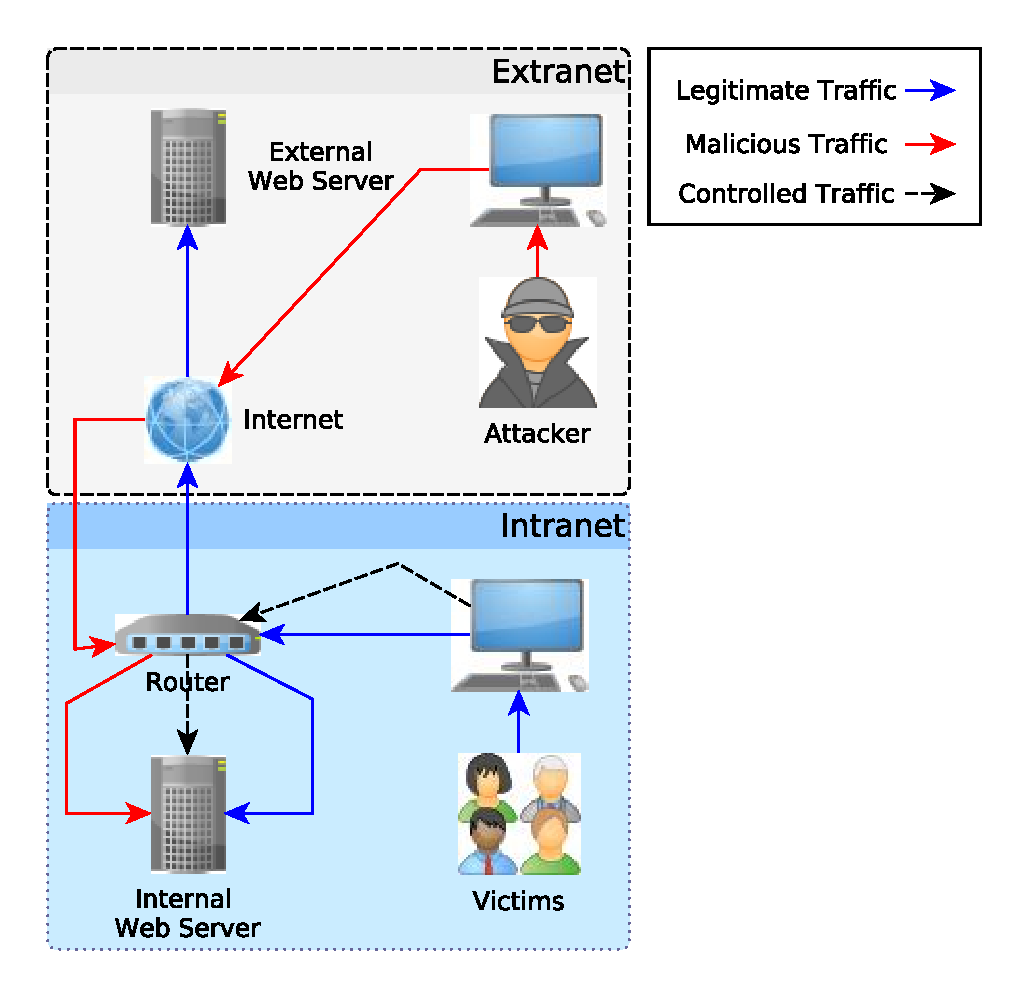
\includegraphics[width=9cm]{figures/ch2/scenario.eps}
     \caption{Scenario to reproduce legitimate traffic, flood and port scan.}
     \label{fig:2.01}
\end{figure}

In many organizations the web based traffic is predominant, since most of corporate services are  web pages, customized web-based systems and cloud services. It is possible to characterize the traffic of a Dynamic Host Configuration Protocol (DHCP) service as an example of legitimate associated with the application layer, as well as it would be possible to classify seasonal and controlled traffic as legitimate traffic. For malicious traffic, three types of networks attacks are evaluated: synflood, fraggle and port scan. Here we refer to port scan as an attack, according to \cite{ahmed2016survey, moustafa2019holistic}, however it is one approach usually adopted for acquire information in order to perform an attack. These attacks are reproduced using well-known security tools, such as Nmap\footnote{http://nmap.org} for port scan, Metasploit\footnote{http://www.metasploit.com} for synflood and Hping\footnote{http://hping.org} to lead the fraggle attack.

A network traffic log is commonly formed by timestamp, protocol, source IP address, source port, destination IP address, destination port and additional information, according to the type of the used transport protocol. The following TCP traffic log is presented in order to exemplify the collected data:
\newline
\newline
\texttt{\justify21:00:34.099289 IP 192.168.1.102.34712 > 200.221.2.45.80: Flags [S], seq 2424058224, win 14600, options [mss 1460, sackOK,TS val 244136 ecr 0,nop,wscale 7], length 0}
\newline

and the following to exemplify UDP traffic log: 
\newline
\newline
\texttt{\justify21:24:42.484858 IP 192.168.1.102.68 > 192.168.1.1.67: BOOTP/DHCP, Request from 00:26:9e:b7:82:be, length 300}
\newline 

In the proposed framework, the goal is to detect the anomalies only taking into account the traffic profile, i.e. specific information such as origin or destination IP, behavioral pattern or content of the attack are not considered. Therefore, IP spoofing or data encryption would not cause impact to the proposed approach and evaluation, since our proposal only relies on the timestamp (for sequencing) and destination port number.

\subsection{Modeling Data}
\label{sec:2_ModelingData}

By modeling the data set as a signal superposition, the network traffic ($\pmb{X}$) can be characterized as a mixture of two components: legitimate traffic ($\pmb{U}$) and malicious traffic ($\pmb{N}$), according to the following expression:

\begin{equation}\label{eq:2.01}
	\pmb{X}^{(q)} = \pmb{U}^{(q)} + \pmb{N}^{(q)},
\end{equation}
where $q$ represents the $q$-th time frame, which is a time aggregation of network traffic. The matrix $\pmb{X}^{(q)} \in \mathbb{R}^{M \times N}$ consists of \emph{M} rows and \emph{N} columns, where each row represents a communication port, and each column represents time bins of a defined size, such as one minute. Each element $x_{m,n}^{(q)}$ stands for the number packets that appears at $n$-th minute for the port $m$, during the $q$-th time frame.

The legitimate traffic $\pmb{U}^{(q)}$ is characterized by user's ordinary operations and by legitimate traffic that are automatically generated for network management and for background services. The access to web pages by users or the name resolution by means of the Domain Name System (DNS) are examples of legitimate traffic generated by user operations, as can be seen in Figure \ref{fig:2.03}, which depicts the legitimate traffic simulated to reproduce user's operations during the experiments.

\begin{figure}[h!]
     \centering 
     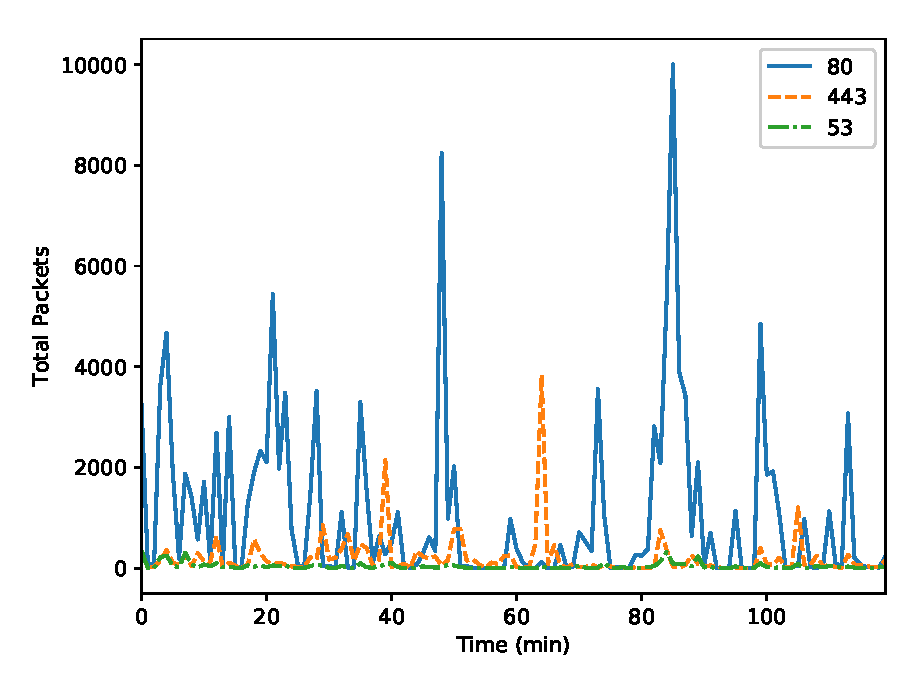
\includegraphics[width=11cm]{figures/ch2/user_traffic.eps}
     \caption{Traffic from user's operations.}
     \label{fig:2.03}
\end{figure}

The Figure \ref{fig:2.04} depicts an example of legitimate traffic of user independent operations, by means of traffic to ports 67 and 68, where it is possible to observe a low amount of packets. The acquisition of logical IP network address by means of DHCP is an example of legitimate traffic not associated with a user, where independently of any user operation, the machine receives an IP address, since it is configured to automatically perform a DHCP address request. 

\begin{figure}[h!]
     \centering 
     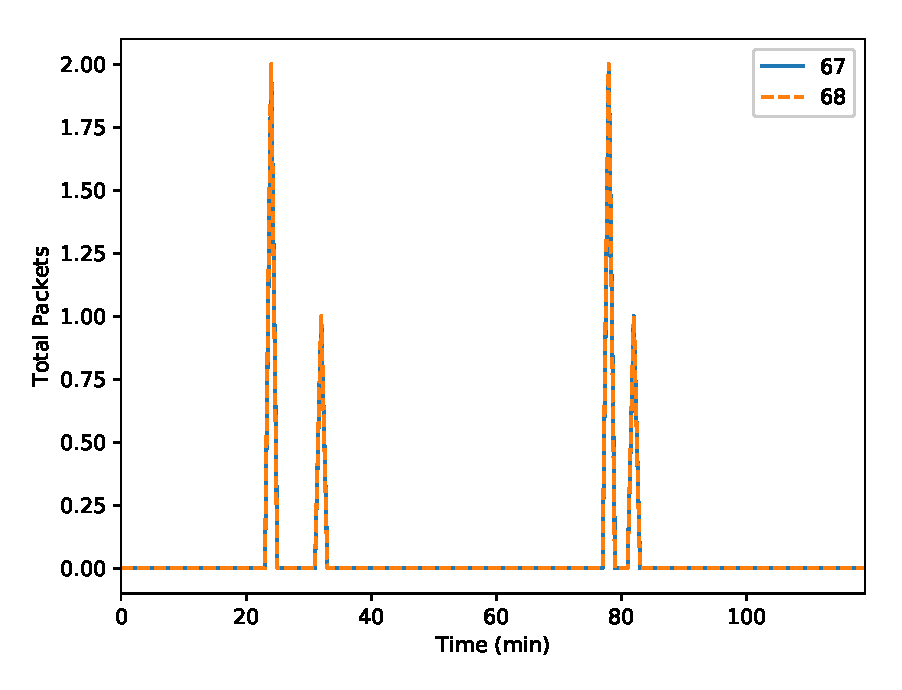
\includegraphics[width=11cm]{figures/ch2/auto_traffic.eps}
     \caption{Network traffic of user independent operations for network management.}
     \label{fig:2.04}
\end{figure}

The traffic coming from a malicious activity, i.e. port scanning, synflood or fraggle attacks, is represented by the matrix $\pmb{N}^{(q)}$. We define that if the rank of $\pmb{X}^{(q)}$ is not zero, according to $\#\pmb{X}^{(q)} \neq 0$, which denotes that the rank of the $q$-th $\pmb{X}$ is different of 0, then there is malicious traffic in the evaluated time frame $q$. On the other hand, if the $\#\pmb{X}^{(q)} = 0$, then there is no malicious traffic in time frame $q$. We show how to detect the $\#\pmb{X}^{(q)}$, given only the matrix $\pmb{X}^{(q)}$, in order to identify malicious traffic.

\subsection{Synflood, Fraggle and Port scan}
\label{sec:2_SynfloodFraggleandPortscan}

The network attacks evaluated by this work are: synflood, fraggle and port scan. The first two attacks can be qualified as flood or denial of service (DoS) attacks, while the last one can be qualified as probe or port scanning attack. 

A DoS is an attempt by an attacker to prevent legitimate access to websites by overwhelming the amount of available bandwidth or resources of the computer system. DoS is implemented by either forcing targets to be unavailable through the exploiting of system vulnerabilities, or consuming resources through large amount of network traffic, characterizing flood attacks. Probe attacks scan computer and network systems to collect information about the host, such as open ports, topology, running software or version of technologies, in order to find vulnerabilities.

With respect to the synflood attacks, the attacker sends a large quantity and concurrent successive SYN requests to a target, in order to consume resources and cause a DoS. Figure \ref{fig:2.05} depicts an example of a synflood attack carried out in a real computer network. In an interval of ten minutes, more than 210,000 packets are sent as a synflood attack. This network traffic behavior can be considered an abnormal behavior of network traffic, especially since it is concentrated in a short period of time and presents similar outstanding traffic during the time under attack.

\begin{figure}[h!]
     \centering 
     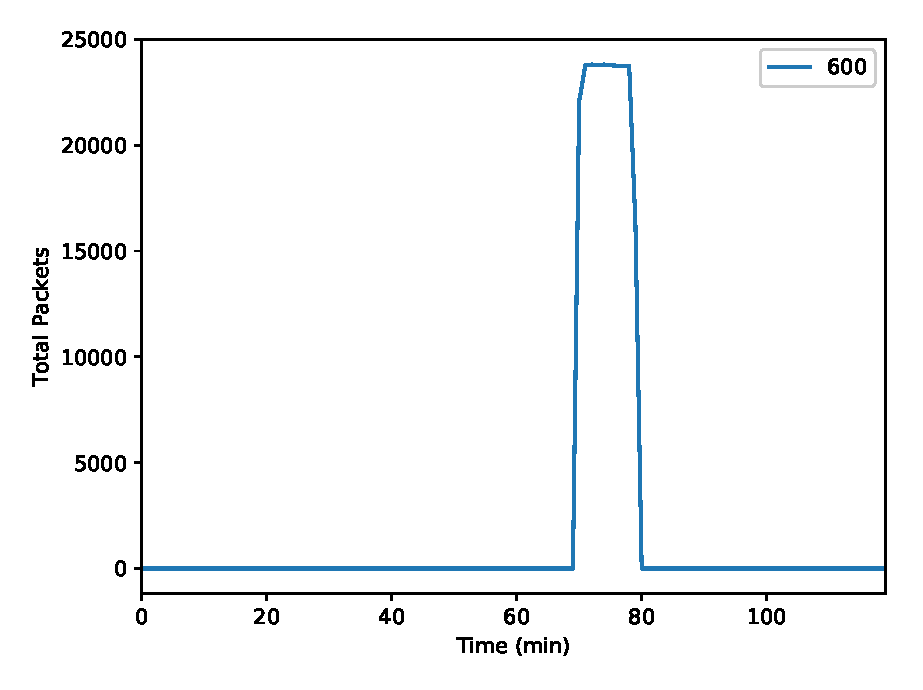
\includegraphics[width=11cm]{figures/ch2/synflood_traffic.eps}
     \caption{A large quantity of SYN requests to a target, in order to cause a DoS.}
     \label{fig:2.05}
\end{figure}

Regarding the fraggle attack, large packets with UDP echo segments are sent to the broadcast address of a network. Every packet is modified to have the source address of the victim, in order to implement the source address spoofing technique. Therefore, each host receives a huge amount of requests UDP echo and all of them replies to the IP address of the victim, causing a packet flooding aiming a DoS. 

The Figure \ref{fig:2.06} depicts an example of the fraggle attack in a real computer network, and shows that more than 6,000,000 malicious packets can be counted in an interval of ten minutes, which can be considered an abnormal network traffic, due to the concentrated traffic in a short period of time and due to the similarity of the outstanding traffic.

The fraggle attack can affect the entire network, since all hosts receive several requests UDP echo and respond with the  Internet Control Message Protocol (ICMP), therefore each host acts as an amplifier of the attack. This part of the fraggle attack is not taken into account in this work, because the victim receives ICMP packets originated from the hosts that are attacked with flooding packet UDP echo. 

\begin{figure}[h!]
     \centering 
     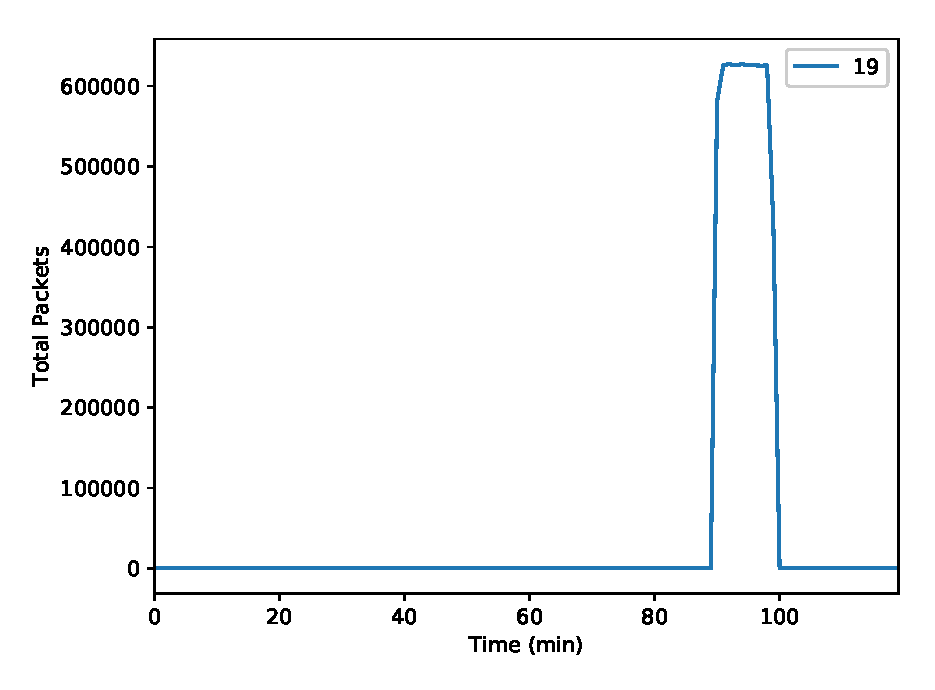
\includegraphics[width=11cm]{figures/ch2/fraggle_traffic.eps}
     \caption{Large amount of “UDP echo” requests and replies, causing packet flooding.}
     \label{fig:2.06}
\end{figure}

Port scan is the attempt to establish a connection to TCP and UDP ports to identify what services are running or are in the listening state. There are several available port scanning techniques, including: TCP SYN scan, TCP ACK scan and UDP scan. This work evaluates the use of TCP SYN scan and UDP scan. 

In TCP SYN scan, a SYN packet is sent to the destination and two types of responses may occur: SYN/ACK or RST/ACK. In the first case, the destination port is in the listening state, in the second case, the destination port is not listening. At the end of each port scanning, a RST/ACK packet is sent by the system that is performing the port scan. Therefore, a full connection or a complete three-way handshake is never established, which makes the detection of the attack sender more difficult, and requires approaches able to identify probe attacks without connection establishment.

The UDP scan technique sends UDP packets to the destination port, and if it responds with a \emph{ICMP port unreachable} message, then it indicates that the scanned port is closed. On the other hand, if a message is not received, then the port is considered as open.

\begin{figure}[h!]
     \centering 
     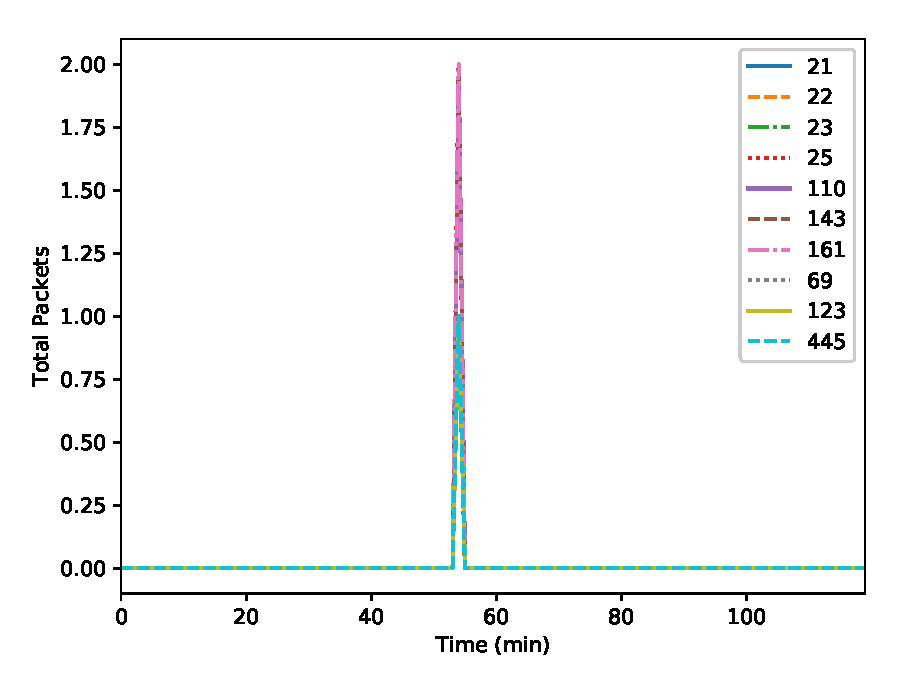
\includegraphics[width=11cm]{figures/ch2/portscam_traffic.eps}
     \caption{Connection attempts in order to identify active ports.}
     \label{fig:2.07}
\end{figure}

Figure \ref{fig:2.07} depicts an example of port scan attack in a real computer network. We simulated a traffic with two packets for each TCP port and one UDP packet to each port. The incoming and outgoing packets analysis, for each port, shows the high correlation and similarity of TCP and UDP traffic during the simulated port scan attack.

\subsection{The DARPA Data set}
\label{sec:2_Darpadata set}

The DARPA 1998 data set\footnote{https://www.ll.mit.edu/ideval/data/} includes 7 weeks of sniffed traffic saved into raw TCPDUMP packet data, from inside and outside origins, with labeled attacks. The attacks in this data set can be grouped into: denial-of-service (DoS); remote to local (R2L), which is characterized by unauthorized access from a remote machine; user to root (U2R), which is characterized by unauthorized access to local super-user privileges; and probe attack. Since the proposed approach focus on flood and probe attack, the analysis concentrates on the attacks of the DARPA 1998 data set that present behaviors similar to flood or probe attack. 

The most cases of DoS of DARPA 98 focus on exploit system vulnerabilities instead of on flooding attack. One example is the occurrence of a neptune attack which sends 20 SYN packets, what is a behavior that differs of the expected flooding attack behavior. Therefore, there were selected the cases that simulates several network traffic or numerous connection requests, also known as flooding attack \cite{ahmed2016survey, osanaiye2016distributed}, and the cases that scan ports sending just a few packets. From the simulated probe attacks, we select the cases that rely on TCP or UDP connections.

The data modeling follows the method described by the Subsection \ref{sec:2_ModelingData}, with time frames of 20 minutes, packet aggregation counting by minute and considering the traffic to the following ports: 20, 21, 22, 23, 25, 79, 80, 88, 107, 109, 110, 113, 115, 143, 161, 389, 443.

\section{Proposed Framework for Detection and Identification of Network Attacks}
\label{sec:2_prop_getv}

According to the overview depicted in Figure \ref{fig:2.08}, we present in this section the proposed framework for detection and identification of network attacks. 

In Subsection \ref{sec:2_prop_LargestEigenvaluebyTimeFrames} we present the steps for extraction of the largest eigenvalue for each $q$-th time frame. Next, in Subsection \ref{sec:2_mos} are presented the mathematical concepts and examples of state-of-the-art MOS schemes, and how to apply the eigenvalues on the MOS scheme in order to detect the attack. In Subsection \ref{sec:2_prop_EigenvalueAnalysis}, we present the eigenvalue analysis to identify the time frames detected as under attack, and the Subsection \ref{sec:2_prop_EigensimilarityAnalysis} describes the similarity analysis evaluated for detailed attack identification.

\begin{figure}[h!]
	\centering
     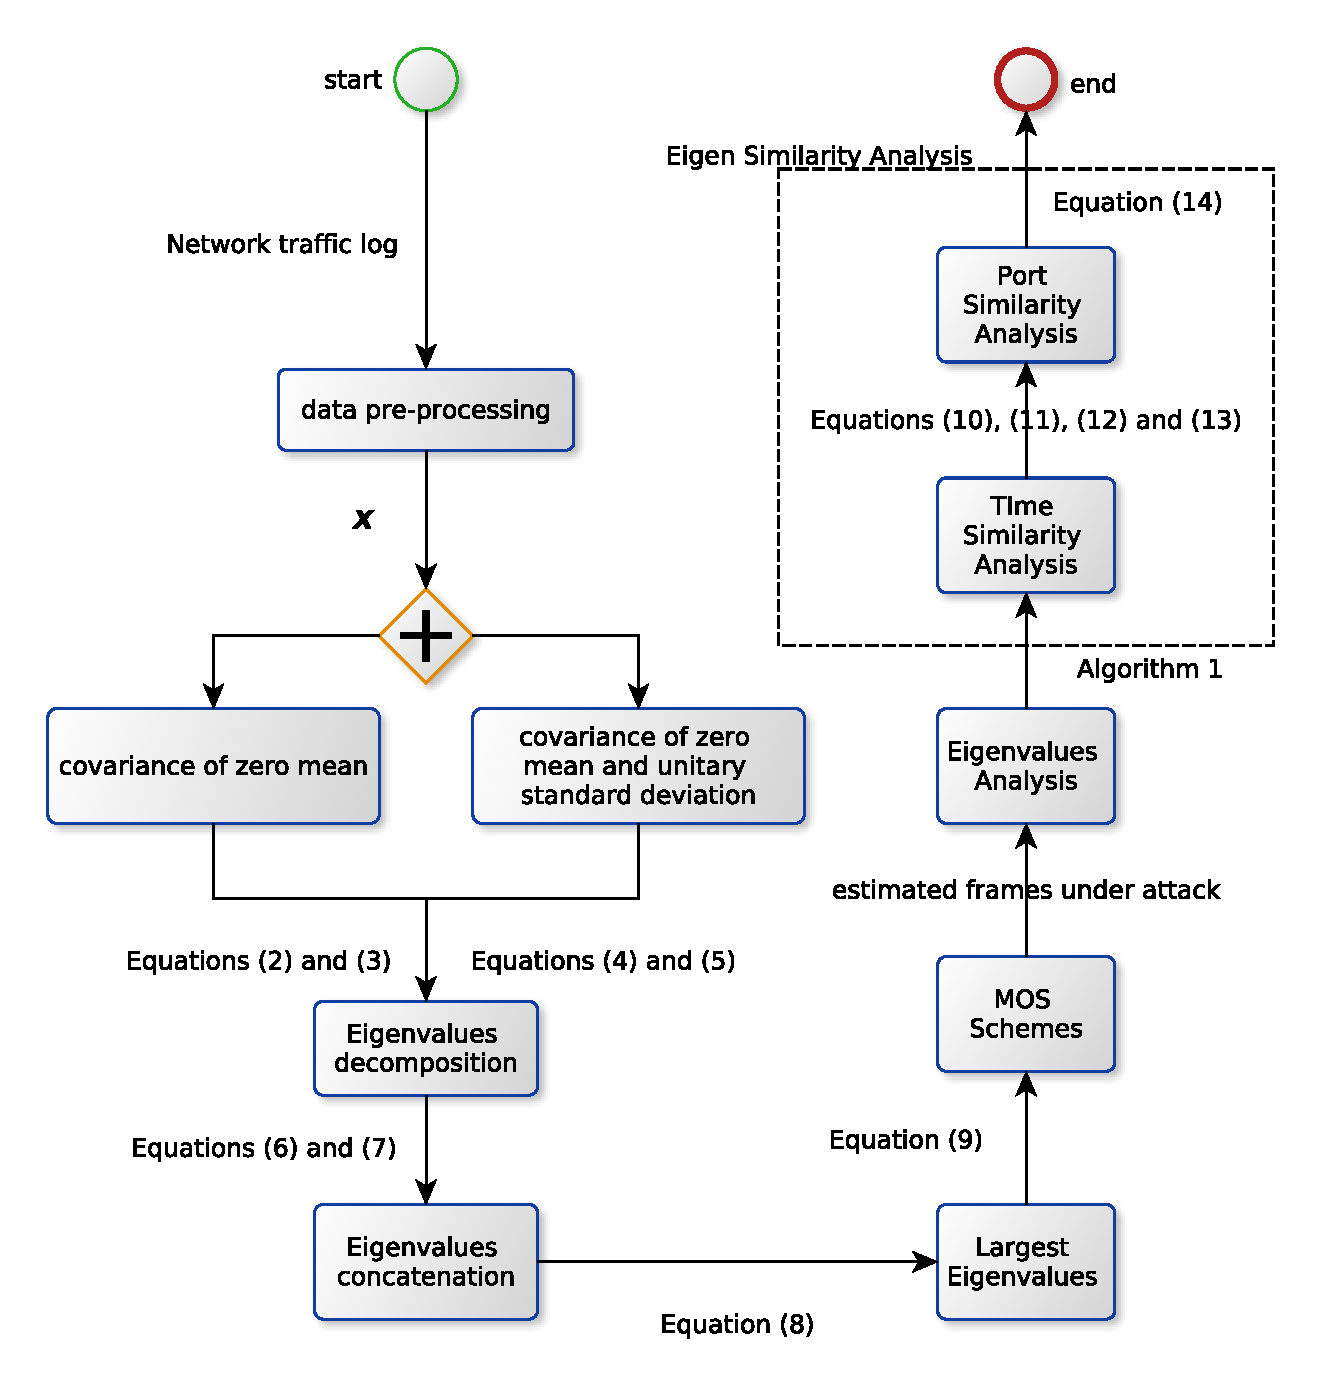
\includegraphics[width=12cm]{figures/ch2/mos_eigen_similarity.eps}
     \caption{Overview of the framework for detection and identification of network attacks.}
     \label{fig:2.08}
\end{figure}

\subsection{Largest Eigenvalue by Time Frames}
\label{sec:2_prop_LargestEigenvaluebyTimeFrames}

The proposed attack detection algorithm starts by the data preprocessing of a network traffic log containing IP, ports and timestamp of senders and receivers. During this step, the desired information is extracted in order to count packets according to the destination ports by time. Subsequently, this information is grouped by minutes and by time frames.

With the data grouped into $Q$ time frames, the framework is initially applied to each matrix $\pmb{X}^{(q)} \in \mathbb{R}^{M\times{N}}$, with $q = 1, \ldots, Q$. According to Subsection \ref{sec:2_ModelingData}, $q$ represents the $q$-th time frame of aggregated network traffic. The matrix $\pmb{X}^{(q)} \in \mathbb{R}^{M \times N}$ consists of \emph{M} network ports and \emph{N} time bins. We adopt time bins with 1 minute of aggregated traffic and time frames with 20 observations. We assume that the count of ports is defined according to $M < N$, and adopt 17 network ports for our evaluation. Hence, we have $\pmb{X}^{(q)} \in \mathbb{R}^{17\times{20}}$ and each element $x_{m,n}^{(q)}$ stands for the number of packets at $n$-th minute for the port $m$, during the $q$-th time frame.

The time frame size is an important concern to define the sampling size for estimating the sample covariance matrix and the eigenvalue decomposition, considering that if the sample size \emph{N} is small and the number of variables \emph{M} is large, the empirical estimators of covariance and correlation can be unstable and the empirical estimate of the covariance matrix becomes singular, i.e. it cannot be inverted to compute the precision matrix. 

However, high-dimension, low-sample-size (HDLSS) data are emerging in many areas, such as genetic, imaging, text classification, finance and face recognition. Thus, many methods of shrinkage and regularization have been proposed to improve the stability for estimation of the covariance matrix \cite{chen2011robust} and eigenvalues \cite{yata2010effective}.

According to flood and port scan attacks' behavior, flood attacks and port scan attacks can be characterized as covariance aware attack \citep{jin2004covariance} and correlation aware attack \citep{lakhina2005mining}, respectively. These characteristics are substantiated by the results obtained through the analysis based on sample covariance of zero mean variables and on covariance of zero mean and unitary standard deviation variables, described in Section \ref{sec:2_experimentalresults}.

The results in Section \ref{sec:2_experimentalresults} show that the main components of flood attacks are dominated by the variables with more variance and that the traffic associated with port scan attack does not generate many logs, however, it presents high covariance of zero mean and unitary standard deviation variables.

Therefore, to detect flood attacks, it is necessary to calculate the sample covariance matrix $\hat{\pmb{R}}_{yy}^{(q)}$ of the zero mean samples given by

\begin{equation}
\label{eq:2.02}
\pmb{y}_{m}^{(q)} = \pmb{x}_{m}^{(q)} - \bar{\pmb{x}}_{m}^{(q)}.
\end{equation}

The set of obtained vectors $\pmb{y}_{m}^{(q)}$ composes the zero mean matrix $\pmb{Y}^{(q)}$, then the sample covariance matrix $\hat{\pmb{R}}_{yy}^{(q)}$ can be calculated as follows

\begin{equation}\label{eq:2.03}
\hat{\pmb{R}}_{yy}^{(q)} = \frac{1}{N}\pmb{Y}^{(q)}\pmb{Y}^{(q)^{\rm T}}.
\end{equation}

For the detection of the port scan attack, the main components are not dominated by the variables with large variance. Moreover, the port scan traffic presents a highly correlated network traffic between the monitored ports. In order to exploit such structure, we compute the sample covariance $\hat{\pmb{R}}_{zz}^{(q)}$ whose variables have zero mean and unitary standard deviation as follows

\begin{equation}
\label{eq:2.04}
\pmb{z}_{m}^{(q)} = \frac{\pmb{x}_{m}^{(q)} - \bar{\pmb{x}}_{m}^{(q)}}{\pmb{\sigma}_{m}^{(q)}}.
\end{equation}

The set of vectors $\pmb{z}_{m}^{(q)}$ composes the matrix $\pmb{Z}^{(q)}$, then the sample covariance matrix $\hat{\pmb{R}}_{zz}^{(q)}$ can be calculated via 

\begin{equation}\label{eq:2.05}
\hat{\pmb{R}}_{zz}^{(q)} = \frac{1}{N}\pmb{Z}^{(q)}\pmb{Z}^{(q)^{\rm T}}.
\end{equation}

Once the $\hat{\pmb{R}}_{yy}^{(q)}$ and $\hat{\pmb{R}}_{zz}^{(q)}$ have been obtained for flood and port scan detection, respectively, and since the next steps are the same for both sample covariance matrices, we refer to $\hat{\pmb{R}}_{yy}$ and $\hat{\pmb{R}}_{zz}$ as a matrix $\hat{\pmb{R}}$. Therefore, the following step of the algorithm is the eigenvalue decomposition (EVD), calculated according to (\ref{eq:2.06}), in order to obtain the vector of eigenvalues $\pmb{e}^{(q)}$ associated with each matrix, according to (\ref{eq:2.06}).

\begin{equation}\label{eq:2.06}
\hat{\pmb{R}}^{(q)} = \pmb{V}^{(q)}\pmb{\Lambda}^{(q)}\pmb{V}^{(q)^{\rm T}},
\end{equation}

\begin{equation}\label{eq:2.060}
\pmb{e}^{(q)} = \rm diag(\pmb{\Lambda}^{(q)}),
\end{equation}

where the operator diag$(\cdot)$ extracts the main diagonal of a matrix.

The eigenvalues should be sorted in descending order, i.e., $\lambda_{1}^{(q)} > \lambda_{2}^{(q)} > \lambda_{3}^{(q)} > ... > \lambda_{m}^{(q)}$. Therefore, the largest eigenvalue of the $q$-th time frame evaluated for the attack detect is given by $\lambda_{1}^{(q)}$.

The concatenation of the eigenvalues vector $\pmb{e}^{(q)}$ for $q = 1, \ldots, Q$ is represented by

\begin{equation}\label{eq:2.07}
\pmb{E} =
\begin{bmatrix}
  \lambda_1^{(1)} & \lambda_1^{(2)} & \lambda_1^{(3)} & \cdots & \lambda_1^{(Q)} \\
  \lambda_2^{(1)} & \lambda_2^{(2)} & \lambda_2^{(3)} & \cdots & \lambda_2^{(Q)} \\
  \lambda_3^{(1)} & \lambda_3^{(2)} & \lambda_3^{(3)} & \cdots & \lambda_3^{(Q)} \\
  \vdots & \vdots & \ddots & \vdots  \\
  \lambda_m^{(1)} & \lambda_m^{(2)} & \lambda_m^{(3)} & \cdots & \lambda_m^{(Q)} \\
\end{bmatrix}.
\end{equation}

Note that since $\lambda_1^{(q)} > \lambda_2^{(q)} > \lambda_3^{(q)} > \cdots > \lambda_{m-1}^{(q)} > \lambda_m^{(q)}$, then the first line of the matrix $\pmb{E}$ contains the largest eigenvalues of each $q$-th time frame, which is the Greatest Eigenvalue Time
Vector (GETV) \cite{tenorio2013greatest}, denoted as 

\begin{equation}\label{eq:2.08}
\pmb{e}_{\rm max} = [ \lambda_1^{(1)}, \lambda_1^{(2)} ... \lambda_1^{(Q)}]
\end{equation}


\subsection{Model Order Selection (MOS)}
\label{sec:2_mos}

The model order selection is a key point in many digital signal processing applications, including radar, sonar, communications, channel modeling, medical imaging, among others \cite{da2011subspace, da2011multi, xiong2017bayesian}. MOS allows analysis of reduced data set, through separating noise components of the main components, for example. Moreover, the model order is crucial for many parameter estimation techniques \cite{da2007enhanced, da2009comparison}, since the amount of parameters to be estimated depends on the model order.

The model selection procedure chooses the ``best'' model of a finite set of models, according to some criteria \cite{rajan1997model}. Therefore, given some data set, it is chosen a model which was evaluated as the best model to describe the specified data set.

The state of the art regarding estimation techniques of model order based on eigenvalues includes: Akaike's Information Theoretic Criterion - AIC \cite{akaike1974new,wax1985detection}; Minimum Description Length - MDL \cite{barron1998minimum,wax1985detection}; Efficient Detection Criterion - EDC \cite{zhao1986detection}; Stein's Unbiased Risk Estimator - SURE \cite{ulfarsson2008rank}; RADOI \cite{radoi2004new} and Exponential Fitting Test - EFT \cite{grouffaud1996some, quinlan2006model, david2011blind}.

In AIC, MDL and EDC techniques, the information criterion is a function of the geometric mean $g(k)$ and the arithmetic mean $a(k)$ relating to smaller $k$ eigenvalues, where $k$ is a candidate value for the model order $d$ \cite{da2009comparison}.

Basically, the difference between the AIC, MDL and EDC schemes is the penalty function $p(k, N, \alpha)$, so these techniques can be written in general as \cite{da2009comparison}:

\begin{equation}\label{eq:eq1}
  \hat{d} = \argmin\limits_k \hspace{1 mm} J(k), 
\end{equation}

where

\begin{equation}\label{eq:eq2}
  J(k) = -N(\alpha - k) \hspace{1 mm} {\rm log} \hspace{1 mm} (g(k)/a(k)) + p(k,N,\alpha),
\end{equation}

where $\hat{d}$ is an estimate $d$ of the model order, $N$ is the number of samples, $\alpha = M$ and means the number of variables of the problem, and $0 \leqslant k \leqslant min[M, N]$. 

Penalty functions for AIC, MDL and EDC are given by the Table \ref{tab:mos_penalty_functions}.

\begin{table}[h!]
  \centering
  \caption{Penalty functions for the schemes AIC, MDL and EDC}
  \label{tab:mos_penalty_functions}
  \begin{tabular}{*2c}
	\toprule
	\textbf{Scheme} &  \textbf{Penalty function} \\
	\textbf{} &  $p(k,N,\alpha)$ \\
	\midrule
    AIC	& $k(2\alpha - k)$ \\
    MDL	& $0.5k(2\alpha - k) \hspace{1 mm} {\rm log} (N)$ \\
    EDC	& $0.5k(2\alpha - k)\sqrt{N\hspace{1 mm}\rm ln(\rm ln N)}$ \\
    \bottomrule
  \end{tabular}
\end{table}

The Exponential Fitting Test (EFT) can effectively be used in cases where the number of samples $N$ is small. This technique is based on observations of data contaminated only with white noise, where the profile of eigenvalues can be approximated by an exponential decaying \cite{grouffaud1996some}.

Given $\lambda_i$ be the i-th eigenvalue, the exponential model can be expressed by:
\begin{equation}\label{eq:eq3}
  E\{\lambda_i\} = E\{\lambda_1\} \cdot q(\alpha,\beta)^{i-1},
\end{equation}

where $E\{\cdot\} $ is the expectation operator, and it is considered that the eigenvalues are ordered in the that $\lambda_1$ represents the largest eigenvalue. The term $q(\alpha, \beta)$ is defined as:

\begin{equation}\label{eq:eq4}
  q(\alpha,\beta) = \exp\left\{-\sqrt{\frac{30}{\alpha^2 + 2} - \sqrt{\frac{900}{(\alpha^2 + 2)^2} - \frac{720\alpha}{\beta(\alpha^4 + \alpha^2 - 2)}}} \right\},
\end{equation}

where $0 < q(\alpha,\beta) < 1$. According to \cite{quinlan2006model}, if $M \leq N$, then $\beta = N$.

Traditionally, the MOS schemes are applied for the eigenvalues, that are the vector $\pmb{e}^{(q)}$ when considering the application of MOS schemes for Eigensimilarity. However, the goal of our proposal is to detect the variations of the eigenvalues for different values of $q$. 

Instead of using a certain $q$, the proposed approach applies MOS schemes for a vector of the largest eigenvalues of each $q$-th time frame, in order to identify variations and estimate the model order $\hat{d}$, which is the estimated number of time frames under attack. Therefore, $\pmb{e}_{\rm max}$ is sorted in descending order, producing $\sim\pmb{e}_{\rm max}$, that is used as input parameter for MOS schemes, according to $\hat{d} = \rm{MOS}(\sim\pmb{e}_{\rm max})$. Note that some MOS schemes may also require the number of minutes that compose a time frame, as $\hat{d} = \rm{MOS}(\pmb{e}_{\rm max},\emph{Q})$.

In our previous work \cite{tenorio2013greatest}, the accuracy of AIC, MDL, EDC, RADOI, EFT and SURE schemes are evaluated for synflood and port scan attack detection, showing that EDC and EFT are effective for detecting this kind of attacks. The present work extends that evaluation to also analyze the effectiveness of the listed MOS schemes for fraggle attack detection, as shown in Section \ref{sec:2_experimentalresults}.

\subsection{Eigenvalue Analysis}
\label{sec:2_prop_EigenvalueAnalysis}

After applying the MOS schemes to the vector $\sim\pmb{e}_{\rm max}$, we obtain the rank estimate of the $\#\pmb{X}$. For instance, in the case of fraggle, synflood and ports can, if $\hat{d} = 1$, then $\#\pmb{X} = 1$ indicate a estimate of rank 1 for $\pmb{X}$, which means that during the during the $Q$ time frames one time frame $q$ is under attack. However, if $\hat{d} = 0$, then $\#\pmb{X} = 0$, and this means that none of the $Q$ time frames is under attack. Note that $\hat{d}$ can be greater than 1, indicating the presence of more than one attacked time frame.

In Subsection \ref{sec:2_mos}, we obtained only if $\hat{d} = 1$ or $\hat{d} = 0$, estimating the number of time frames under attack. However, if $\hat{d} > 1$, the MOS schemes does not identify the $q$-th attacked time frames. The identification of the $q$-th time frame under attack can be carried out through an eigenvalues analysis.

The largest eigenvalue analysis for estimating the $q$-th time frames that are under attack can be expressed according to Algorithm \ref{alg:2.01}, where $\rm{\hat{\pmb{q}}}_{\rm max} \in \mathbb{R}^{\hat{d}}$ denotes a vector of the $q$-th time frames under attack, which is the $q$-th indexes corresponding to the $\hat{d}$ largest eigenvalues of $\pmb{e}_{\rm max}$. Algorithm \ref{alg:2.01} initially identifies the largest value of $\pmb{e}_{\rm max}$, according to Line 3 of Algorithm \ref{alg:2.01}, and its correspondent index, according to Line 7. Subsequently, the largest value is removed of $\pmb{e}_{\rm max}$, according to Line 11 of Algorithm \ref{alg:2.01}, and a new iteration is performed until $\pmb{e}_{\rm max} = []$.

\begin{algorithm}
	\label{alg:2.01}
	\SetAlgoLined
	\KwResult{$\rm{\hat{\pmb{q}}}_{\rm max}$}
	Given $f = 1$\;
	\While{$f < \hat{d}$}{
		$q_{\rm value} = \operatorname*{argmax}_{\lambda}  \hspace{1 mm} \pmb{e}_{\rm max}$\;
		$i = 1$\;
    	\While{$i < Q$}{
    		\If{$\pmb{e}_{\rm max}^{(i)} == q_{\rm value}$}{
    			$\hat{\pmb{q}}_{\rm max}^{(f)} = i$\;
    		}
    		$i = i + 1$\;
    	}
    	$\pmb{e}_{\rm max} \rightarrow \hat{\pmb{q}}_{\rm max}^{(f)}$\;
		$f = f + 1$\;
	}
	\caption{Detection of Time Frames Under Attack}
\end{algorithm}

After the estimation of the $\rm{\hat{\pmb{q}}}_{\rm max}$ time frames under attack, it is necessary to obtain more details of the detected Attacks, such as the $n$-th minutes when the attacks happened and the $m$-th network ports that were attacked. To deal with this problem, the adoption of a similarity analysis between legitimate traffic and the traffic of time frames estimated as under attack is evaluated, analyzing the effectiveness of cosine similarity to highlight abnormalities inserted by network traffic attacks. 

\subsection{Principal Eigenvector Similarity Analysis}
\label{sec:2_prop_EigensimilarityAnalysis}

The eigenvector corresponding to the eigenvalue of largest magnitude is called the principal eigenvector or dominant eigenvector. Cosine similarity calculates the cosine of the angle between two vectors, which represents the similarity of values between the selected vectors. Therefore, cosine similarity can be used to evaluate the difference between the principal eigenvector $\pmb{V}^{(q)}$ against the principal eigenvector of one time frame detected as under attack, in order to analyze similarity changes between the principal eigenvectors with the largest variance caused by the insertion of anomalous traffic \cite{Lee2013} in a time frame.

The cosine similarity is a measure between two vectors and does not consider the distance between points or features of a vector. Therefore, the computed angle between eigenvectors does not reveal element-wise distance neither the contribution of each component for the measured distance, but can be used to identify the principal eigenvector of observations that deviates from a reference principal eigenvector and can identify network attacks. After the identification of the time under attack by means of the cosine similarity between principal eigenvectors, the cosine similarity can also be applied for identification of components that insert the deviation between the principal eigenvectors, according explained in subsection \ref{sec:2_prop_PortSimilarityAnalysis}.

This subsection describes the proposed principal eigenvector similarity analysis for detailed attack identification, in complement to the attack estimation carried out through MOS schemes and eigenvalue analysis. In Subsection \ref{sec:2_prop_TimeSimilarityAnalysis} we present the principal eigenvector similarity analysis for identification of time under attack. Next, in Subsection \ref{sec:2_prop_PortSimilarityAnalysis}, we show how to apply the principal eigenvector similarity analysis in order to identify network ports under attack.

\subsubsection{Time Similarity Analysis}
\label{sec:2_prop_TimeSimilarityAnalysis}

For principal eigenvector similarity analysis, we evaluate the cosine similarity in order to identify lacks of similarity between legitimate and malicious traffic, as follows:

\begin{equation}\label{eq:2.11}
s_n = \frac{\abs{\pmb{v}^{(q)} \cdot \pmb{v}_{(n)}^{(q)}}}{\norm{\pmb{v}^{(q)}}\norm{\pmb{v}_{(n)}^{(q)}}},
\end{equation}
where $s_n$ denotes the absolute similarity degree between the $n$-th minute and the reference principal eigenvector, given by an inner product that measures the cosine of the angle between two vectors, where the $l_2$ norm is denoted by $\norm{\cdot}$ and $\abs{\cdot}$ denotes the absolute value. 

In (\ref{eq:2.11}), the $\pmb{v}^{(q)}$ denotes the principal eigenvector of a selected set of minutes without network attack, according the attack detection described by Algorithm \ref{alg:2.01}, and $\pmb{v}_{(n)}^{(q)}$ is the principal eigenvector obtained after append each target $n$-th minute of traffic that needs the identification of flood and port scan attacks. 

The principal eigenvector $\pmb{v}^{(q)}$ of a time frame $q$ without attack can be computed from (\ref{eq:2.06}) and selected according to the eigenvector corresponding to the largest eigenvalue $\lambda_1^{(q)}$, which is the principal component of the selected time frame $q$. The same calculation shall be performed in order to obtain the target principal eigenvector $\pmb{v}_{(n)}^{(q)}$, calculated from the time frame without attack appended by selected minutes of a time frame estimated as under attack.

Therefore, the principal eigenvector $\pmb{v}^{(q)}$ is calculated from the traffic without attack, in a time frame $q$ composed of $Q$ minutes of legitimate network traffic, estimated as normal by Algorithm \ref{alg:2.01}. For the detailed attack identification, each $\pmb{x}^{(\hat{q})}_{(n)}$ vector of each $n$-th minutes of the estimated $\rm{\hat{\pmb{q}}}_{\rm max}$ time frames shall be individually appended into $\pmb{X}^{(q)}$, as represented by

\begin{equation}\label{eq:2.12}
\pmb{X}_{n} = \{\pmb{X}^{(q)} | \pmb{x}^{(\hat{q})}_{(n)}\}.
\end{equation}

Subsequently, the resultant $\pmb{X}_{(n)}$ is used to obtain $\pmb{v}_{(n)}^{(q)}$, through (\ref{eq:2.06}), for calculating the similarity degree $s_n$, ranging from 0 to 1, for each $n$-th minute. The $s_n$ denotes the absolute similarity degree of the $n$-th minute in comparison to a well-known traffic without attack, detected through MOS schemes and eigenvalue analysis.

We propose three approaches for principal eigenvector similarity analysis, which are the incremental, the individual and the incremental individualized.

The incremental approach for principal eigenvector similarity analysis is based on the incremental appending of network traffic into $\pmb{X}^{(q)}$, where the first evaluation is based on (\ref{eq:2.12}) and the subsequent evaluations are based on (\ref{eq:2.13}), that denotes the appending of the $n$-th minute $\pmb{x}^{(\hat{q})}_{(n)}$ into $\pmb{X_n}$. The incremental approach repeats the (\ref{eq:2.13}) while $n \leq N$ and compute $\pmb{v}^{(q)}$, $\pmb{v}_{(n)}^{(q)}$ and the (\ref{eq:2.11}) for each increment.

\begin{equation}\label{eq:2.13}
\pmb{X}_{n} = \{\pmb{X}_{n} | \pmb{x}^{(\hat{q})}_{(n)}\},
\end{equation}

Figure \ref{fig:2.88} illustrates the network traffic selection for the incremental approach of principal eigenvector similarity analysis, where the $\pmb{X}^{(1)}$ is chosen as reference for similarity analysis of the $m$-th minutes of the time frame $q=3$, where one network attack was previously detected by Algorithm \ref{alg:2.01}. 

%TODO - fix figure that shows s_n > l where should the inverse
\begin{figure}[h!]
     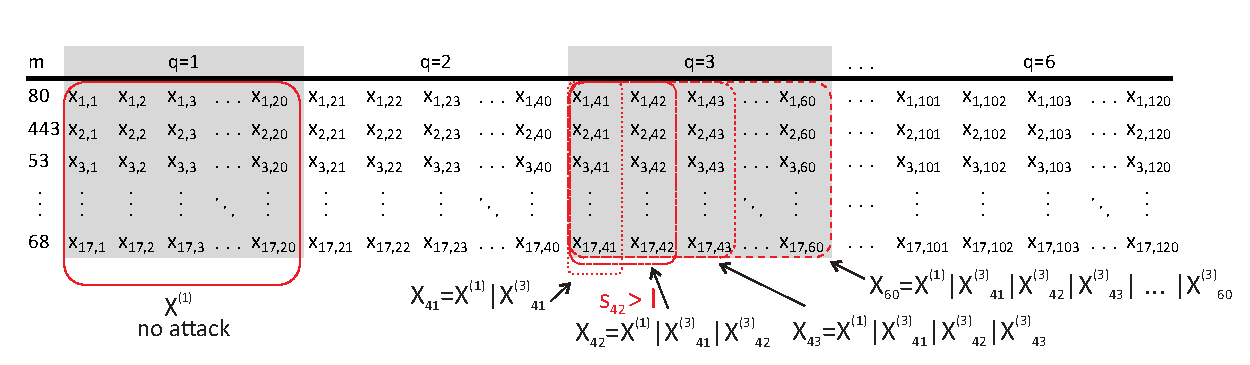
\includegraphics[width=15cm]{figures/ch2/incremental.eps}
     \caption{Traffic selection for incremental approach.}
     \label{fig:2.88}
\end{figure}

For the scenario depicted by Figure \ref{fig:2.08}, the principal eigenvector similarity analysis starts at $\pmb{x}^{(3)}_{(41)}$ and is incrementally performed until $\pmb{x}^{(3)}_{(60)}$, in order to calculate the $s_n$. We assume that $s_n < l$ means an attack identification, according the anomaly on similarity of $s_n$ compared to a defined threshold $l$. 

Therefore, after obtaining the principal eigenvector $\pmb{v}^{(q)}$ and the target principal eigenvector $\pmb{v}_{(n)}^{(q)}$ for principal eigenvector similarity analysis, the $s_n$ is calculated according to (\ref{eq:2.11}). If $s_n = 1$, then the two principal eigenvectors are completely similar and no anomaly is detected. Smaller values of $s_n$ mean less similarity and can indicate an anomaly if $s_n < l$, what denotes that a network attack is identified during the $n$-th minute. 

The (\ref{eq:2.14}) shows how the $s_n$ of each $n$-th minute shall be compared with the threshold $l$ to evaluate if an attack is identified, where

\begin{equation}\label{eq:2.14}
  \hat{\pmb{n}}_{(n)}=\left\{
  \begin{array}{@{}ll@{}}
    1, & \text{if}\ s_n < l \\
    0, & \text{otherwise}
  \end{array}\right.,
\end{equation}
and $\hat{\pmb{n}}_{(n)}$ denotes a vector of $n$-th minutes detected as under attack.

The principal eigenvector similarity analysis can also be applied by means of the individual approach, where each $n$-th minute must be individually appended into $\pmb{X}^{(q)}$, as shown by Figure \ref{fig:2.09}. In the individual approach there is no incremental appending, therefore only individual $n$-th minute are appended to $\pmb{X_n}$, according to (\ref{eq:2.12}), in order to compute $\pmb{v}^{(q)}$, $\pmb{v}_{(n)}^{(q)}$ and the (\ref{eq:2.11}) for individual $n$-th minute.

%TODO - fix figure that shows s_n > l where should the inverse
\begin{figure}[h!]
     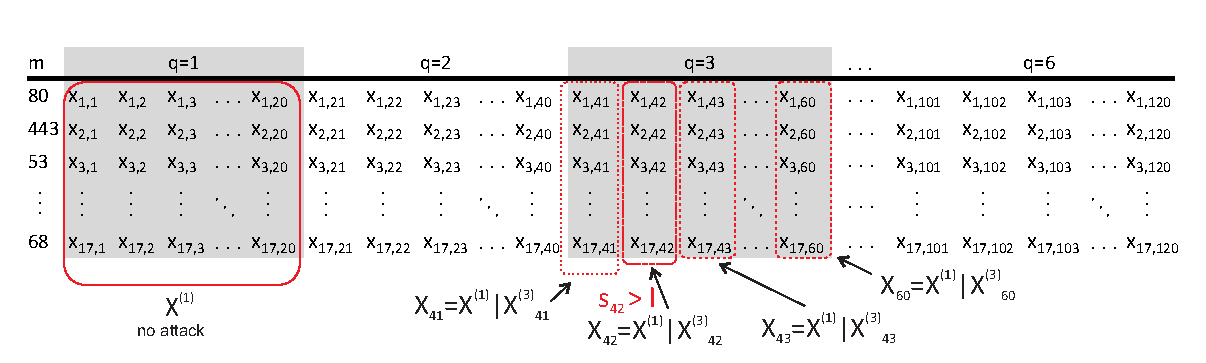
\includegraphics[width=15cm]{figures/ch2/individualized.eps}
     \caption{Traffic selection for individual approach.}
     \label{fig:2.09}
\end{figure}

The incremental and the individual approaches can be combined to obtain the incremental individualized approach, where each minute is incrementally appended into the selected $\pmb{X}^{(q)}$ for obtaining $\pmb{v}_{(n)}^{(q)}$ to compute similarity analysis of the $n$-th minute, until detect the first $n$-th minute under attack, i.e. $s_n < l$. Subsequently, $\pmb{X}_{n-1}$ becomes the new reference of traffic without network attack and each subsequent minute must have its similarity individually evaluated, as shown in Figure \ref{fig:2.22}.

%TODO - fix figure that shows s_n > l where should the inverse
\begin{figure}[h!]
     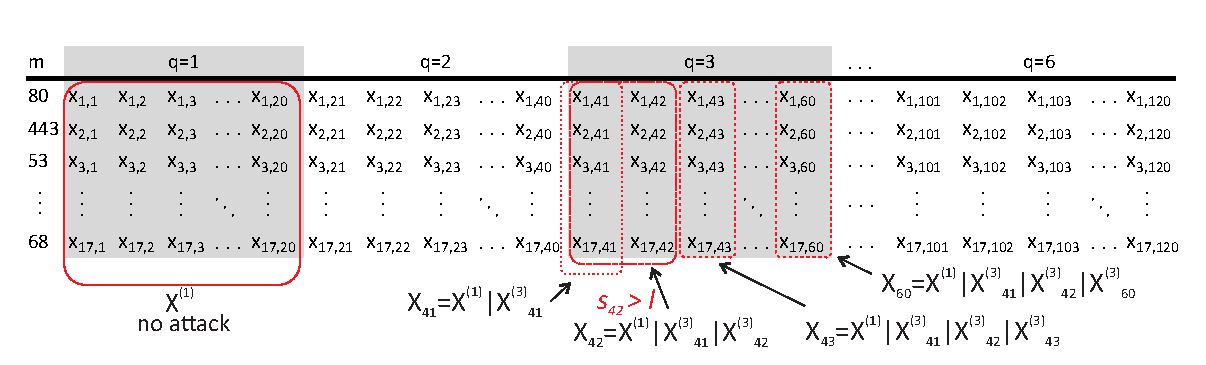
\includegraphics[width=15cm]{figures/ch2/incremental_individualized.eps}
     \caption{Traffic selection for incremental individualized approach.}
     \label{fig:2.22}
\end{figure}

The incremental similarity analysis followed by individual analysis after an attack detection allows to identify the attack period, highlighting the first and last time under attack. This identification is possible due to the similarity variation between the principal eigenvectors, which highlight lacks of similarity when compared the principal eigenvector of a traffic under attack against the principal eigenvector of a traffic with no attack, according to results which are discussed in Section \ref{sec:2_experimentalresults}.

\subsubsection{Port Similarity Analysis}
\label{sec:2_prop_PortSimilarityAnalysis}

Given $\hat{\pmb{n}}$, which is the set of $n$-th minutes under attack, it is still necessary to obtain more details about the identified network attack, such as the network ports that are attacked during each $n$-th minute identified as under attack. Hence, it is also applied the cosine similarity analysis to identify variation of the principal eigenvectors, caused by the insertion of anomalous network traffic by a selected $m$-th port during a $n$-th minute. 

For detection of ports under attack, the last principal eigenvector without attack $\pmb{v}^{(q)}$ shall be used as reference for similarity analysis against the $\pmb{v}_{(n)}^{(q)}$ identified as under attack, and evaluate individually the cosine similarity of each $m$-th port of all $\hat{\pmb{n}}$ minutes. Therefore, $\pmb{v}^{(q)}$ should be calculated from the last $\pmb{X}^{(q)}$ time frame without attack, and $\pmb{v}_{(m,\hat{n})}$ should be calculated from the same traffic appended of all $n$-th minutes until the identified minute under attack, denoted as $\pmb{X}_n$. 

For similarity analysis, each $m$-th port of the last $n$-th minute of $\pmb{X}_n$, denoted as $x_{(m,n)}$, shall be individually replaced by the traffic of the evaluated $m$-th port of the $\hat{n}$-th minute under attack, denoted as $x^{(\hat{q})}_{(m,\hat{n})}$, in order to identify significant variation on similarity caused by the traffic of the $m$-th port. 

This approach for detection of ports under attack via similarity analysis is given by

\begin{equation}\label{eq:2.15}
  \left\{
  \begin{array}{@{}ll@{}}
    x_{(m,n)} = x^{(\hat{q})}_{(m,\hat{n})} \\
    \\
    s_{m,\hat{n}} = \frac{\abs{\pmb{v}^{(q)} \cdot \pmb{v}_{(m,\hat{n})}}}{\norm{\pmb{v}^{(q)}}\norm{\pmb{v}_{(m,\hat{n})}}},
  \end{array}\right.
\end{equation}
where $x^{(\hat{q})}_{(m,\hat{n})}$ denotes the $m$-th port of the selected $n$-th minute and $q$-th time frame identified as under attack and $x_{(m,n)}$ denotes the $m$-th port of the last $n$-th minute of $\pmb{X}_n$, which is used to calculate the $\pmb{v}_{(m,\hat{n})}$ principal eigenvector that contains the traffic of the $m$-th port of the $\hat{n}$-th minute identified as under attack.

Once $\pmb{v}^{(q)}$ and $\pmb{v}_{(m,\hat{n})}$ are obtained, then the $s_{m,\hat{n}}$ similarity degree can be calculated in order to identify if the traffic replacement highlights the addition of anomalous traffic by the evaluated $m$-th port during the $\hat{n}$-th minute previously identified as under attack. 

This procedure should be repeated for each $m$-th target port of $\hat{\pmb{n}}$, in order to individually identify the network ports under attack during each $\hat{q}$-th time frame.


\section{Experiments and Results}
\label{sec:2_experimentalresults}

This section presents the performed experiments and the acquired results for the Eigensimilarity. First, in Section \ref{sec:2_AnalyzedScenario}, the experimental scenario adopted in the evaluation is summarized. Then, in Section \ref{sec:2_largesteigenvaluesanalysis} the results of the largest eigenvalue analysis by time frames for the experimental scenario are shown. In Section \ref{sec:2_MOSSchemesEvaluation} we describe the results of the evaluated MOS schemes for attack detection in the simulated data set. In Section \ref{sec:2_EigenvalueAnalysis} we present the results of the eigenvalue analysis for identification of time frames under attack. In Section \ref{sec:2_EigensimilarityAnalysis} we show the results of similarity analysis for detailed flood and port scan identification for the experimental scenario. In Section \ref{sec:2_DarpaEvaluation} we present the results of the proposed framework for flood and probe attack detection in the DARPA 1998 data set.


\subsection{Experimental Scenario}
\label{sec:2_AnalyzedScenario}

This experiment considers a simulated scenario of a real network monitored during 120 minutes, that are separated into six time frames of twenty minutes. Therefore, as the time of each sampling period is one minute, then $N = 20$. For each time frame $q$, a traffic matrix $\pmb{X}^{(q)} \in \mathbb{R}^{17 \times 20}$ was obtained, as well as a covariance $\hat{\pmb{R}}_{yy}^{(q)} \in \mathbb{R}^{17 \times 17}$ (calculated via (\ref{eq:2.03})) and a sample covariance matrix $\hat{\pmb{R}}_{zz}^{(q)} \in \mathbb{R}^{17x17}$, assuming that $q = 1, 2, 3, 4, 5$ and $6$. 

The simulation started at 21:00h, the first time frame was from 21:00h until 21:20h ($q = 1$), the second was from 21:20h until 21:40h ($q = 2$), the third was from 21:40h to 22:00h ($q = 3$), the fourth was from 22:00h until 22:20h ($q = 4$), the fifth was from 22:20h until 22:40h ($q = 5$), and finally, the sixth was from 22:40h until 23.00h ($q = 6$). During the simulation, the victim made legitimate access, and the attacker performed the following attacks: at 21:54h ($q = 3$) was performed a port scan, at the interval ranging from 22:10h to 22:20h ($q = 4$) a synflood attack was simulated, and at the interval from 22:30h to 22:40h ($q = 5$) a fraggle attack was performed.

\subsection{Largest Eigenvalues Analysis}
\label{sec:2_largesteigenvaluesanalysis}

For the evaluation of MOS Schemes accuracy for flood and port scan detection, the framework defines that it is necessary to obtain the largest eigenvalue of each time frame, through eigen decomposition from a covariance of zero mean variables or covariance matrix of zero mean and unitary standard deviation variables, calculated from the evaluated traffic, as described in Section \ref{sec:2_prop_getv}. 

Through eigenvalue analysis of traffic with flood or port scan attacks, it is possible to visualize a significant difference between the largest eigenvalues and the remain eigenvalues, which can indicate a relationship between an outlier and time frames under attack.

Figure \ref{fig:2.10} depicts the eigenvalues calculated from sample covariance matrix of the network traffic used to evaluate the synflood attack identification. In Figure \ref{fig:2.10}, the largest eigenvalue related to the simulated synflood attack ($q = 4$) stands out significantly from the other eigenvalues.

\begin{figure}[h!]
	\centering
     \includegraphics[width=9cm]{figures/ch2/eigenvalues_synflood.eps} 
     \caption{Eigenvalues of the sample covariance matrix (synflood).}
     \label{fig:2.10}
\end{figure}

Figure \ref{fig:2.11} illustrates the eigenvalues calculated from sample covariance matrix of the matrix used for fraggle attack detection. In Figure \ref{fig:2.10}, the largest eigenvalue related to the simulated synflood attack ($q = 5$) stands out significantly from the other eigenvalues, in accordance with the result shown in Figure \ref{fig:2.10} for the synflood attack analysis.

\begin{figure}[h!]
	\centering
     \includegraphics[width=9cm]{figures/ch2/eigenvalues_fraggle.eps}
     \caption{Eigenvalues of the sample covariance matrix (fraggle).}
     \label{fig:2.11}
\end{figure}

Figure \ref{fig:2.12} depicts the eigenvalues calculated from covariance matrix of zero mean and unitary standard deviation variables, of the network traffic matrix evaluated for port scan detection. As analyzed for the synflood and fraggle attacks, note that the largest eigenvalue, related to this attack ($q = 3$), stands out significantly from the others eigenvalues.

\begin{figure}[h!]
	\centering
     \includegraphics[width=9cm]{figures/ch2/eigenvalues_portscan.eps}
     \caption{Eigenvalues of the covariance matrix of zero mean and unitary standard deviation (port scan).}
     \label{fig:2.12}
\end{figure}

Table \ref{tab:2.03} presents the values of the largest eigenvalues of each time frame $q$-th for port scan, synflood and fraggle detection. 

\begin{table}[h!]
  \centering
  \footnotesize
  \caption{Largest Eigenvalue related to attacks detection}
  \label{tab:2.03}
  \begin{tabular}{ c c c c c }
	\toprule
	\multirow{3}{*}{\textbf{Time Frame} $q$} &\multicolumn{4}{c }{\textbf{Vectors GETV}}\\ 
			\hhline{~----}
		&\textbf{Detection of}	 &\textbf{Detection of}	 &\textbf{Detection of}	 &\textbf{Detection of}\\
		&\textbf{\emph{synflood/fraggle}}	 &\textbf{\emph{synflood}}	 &\textbf{\emph{fraggle}}	 &\textbf{\emph{port scan}}\\
	\midrule
	1 &1887545 &1887545 &1887545 &2,0734 \\
	2 &2341327 &2341327 &2341327 &2,1451 \\
	3 &3213867 &3213867 &3213867 &10,0718 \\
	4 &133238294 &133238294 &731229 &2,1620 \\
	5 &92384021611 &6367983 &92384021611 &2,4253 \\
	6 &708335 &708335 &708335 &1,7948 \\
    \bottomrule
  \end{tabular}
\end{table}

In Table \ref{tab:2.03}, note the significant variation of the eigenvalues associated with attacks, in comparison to the others. At $q = 4$, where the synflood attack occurred, the maximum eigenvalue obtained is approximately 21 times larger than the second one. At $q = 5$, where the fraggle attack occurred, the maximum eigenvalue obtained is about 29,000 times larger than the second one. At $q = 3$, where the port scan attack occurred, the maximum eigenvalue obtained is approximately 4 times larger than the second one. In the last case, for port scan attack detection, although the largest eigenvalue presented no too large variance to the second one, if compared to synflood or fraggle attacks, it clearly deviates from the remaining largest eigenvalues.

These results highlight that all $q$-th time frames where a network attack was simulated, present high significant variance between the largest eigenvalue and the remaining eigenvalues, obtained from sample covariance matrix, for flood detection, or from covariance matrix of zero mean and unitary standard deviation variables, for port scan detection. Therefore, we propose to apply the vector of the largest eigenvalues to MOS schemes in order to evaluate their accuracy for identification of time frames under attack, motivated by the fact that it is relevant to apply MOS schemes to automate the attack detection process, taking into account the characteristics of the evaluated eigenvalues.

\subsection{MOS Schemes Evaluation}
\label{sec:2_MOSSchemesEvaluation}

In \cite{tenorio2013greatest}, we evaluate the accuracy of AIC, MDL, EDC, RADOI, EFT and SURE MOS schemes \cite{da2009comparison,tenorio2013greatest} for synflood and port scan attack detection. In this work we extend that evaluation for fraggle attack detection, applying the same schemes to fraggle attack detection over the traffic presented in Section \ref{sec:2_datamodel}, as results shown in Table \ref{tab:2.04}.

Note that $\hat{d} = 1$, if there is one attack, while $\hat{d} > 1$ indicates more than one attack. An example of this could be seen for attack detection via EFT for traffic containing synflood and fraggle attacks, showing $\hat{d} = 2$, which indicates the presence of two attacks, as expected by the ground truth values $d$ of Table \ref{tab:2.04}. 

\begin{table}[h!]
  \centering
  \footnotesize
  \caption{MOS schemes applied to port scan and flood detection}
  \label{tab:2.04}
  \begin{tabular}{ c c c c c c c c }
	\toprule
	\multirow{2}{*}{\textbf{Type of analysis} $q$} &\multicolumn{6}{c}{MOS schemes (estimated model order $\hat{d}$)} &{(d)}\\ 
			\hhline{~------~}
		&\textbf{AIC} &\textbf{MDL} &\textbf{EDC} &\textbf{RADOI} &\textbf{EFT} &\textbf{SURE}\\
	\midrule
	Detection of synflood \\(presence of attack) &2 &1 &\textbf{1} &5 &\textbf{1} &4 &\textbf{1} \\
	Detection of synflood \\(absence of attack) &1 &1 &\textbf{0} &1 &\textbf{0} &3 &\textbf{0} \\
	\midrule
	Detection of fraggle \\(presence of attack) &1 &1 &\textbf{1} &5 &\textbf{1} &4 &\textbf{1} \\
	Detection of fraggle \\(absence of attack) &1 &1 &\textbf{0} &1 &\textbf{0} &3 &\textbf{0} \\
	\midrule
	Detection of port scan \\(presence of attack) &1 &1 &\textbf{1} &1 &\textbf{1} &9 &\textbf{1} \\
	Detection of port scan \\(absence of attack) &0 &0 &\textbf{0} &1 &\textbf{0} &1 &\textbf{0} \\
	\midrule
	Detection of synflood/fraggle \\(presence of attack) &2 &2 &\textbf{2} &5 &\textbf{2} &5 &\textbf{2} \\
	Detection of synflood/fraggle \\(absence of attack) &1 &1 &\textbf{0} &1 &\textbf{0} &3 &\textbf{0} \\
    \bottomrule
  \end{tabular}
\end{table}

In Table \ref{tab:2.04}, two MOS schemes outperforms from the others, which are EDC and EFT. Efficient Detection Criterion (EDC) and Exponential Fitting Test (EFT) are the most effective schemes, correctly estimating the number of attacks in comparison to the expected values for effective attack detection, as defined by the column of real values in Table \ref{tab:2.04}. The AIC and MDL schemes are satisfactory only for port scan detection, however SURE and RADOI schemes did not show effective results for port scan or flood detection.

Although EDC and EFT presented the same accuracy on the evaluation, the EDC scheme requires less processing time than EFT, which is an important criteria to select EDC as the MOS scheme for flood and port scan detection on the remain experiments.

According to Table \ref{tab:2.04}, EDC and EFT estimated correctly the number of attacks of a time frame vector, indicating that occurred $\hat{d}$ network attacks, but not providing additional details, what highlights the necessity of complementary approaches in order to estimate the time and ports under attack. Hence, we propose apply eigen analysis to estimate the $q$-th time frames under attack and principal eigenvector similarity analysis to estimate the minutes and ports under attack.

\subsection{Eigenvalue Analysis}
\label{sec:2_EigenvalueAnalysis}

According to the results presented in Section \ref{sec:2_largesteigenvaluesanalysis}, the largest eigenvalue stands out significantly from the others eigenvalues of an evaluated $q$-th time frame. This behavior can also be observed in the largest eigenvalues analysis, according to results presented in Table \ref{tab:2.03}, where it is possible to observe that the $\hat{d}$ largest eigen values of the time frames under attacks stand out significantly from the others largest eigenvalues. 

Therefore, we conclude that the $\hat{d}$ largest eigenvalues correspond to the respective $q$-th time frames under attack, which is denoted by $\rm{\hat{\pmb{q}}}_{\rm max}$ and can be calculated according to Algorithm \ref{alg:2.01}.

\subsection{Principal Eigenvector Similarity Analysis}
\label{sec:2_EigensimilarityAnalysis}

In order to analyze the hypotheses $H_1^{(N)}$ and $H_1^{(A)}$, which evaluate if a subspace learned by eigenvalue decomposition can be used to detect and identify network attacks, we propose to apply principal eigenvector similarity analysis to detect time and ports under attack, from each $q$-th time frames under attack defined by $\rm{\hat{\pmb{q}}}_{\rm max}$. Hence, the proposed framework is applied to the time frames where $q=3$, $q=4$ and $q=5$ to respectively evaluate its effectiveness for port scan, synflood and fraggle attack detection.

\subsubsection{Time Analysis}
\label{sec:2_TimeAnalysis}

Three approaches were evaluated for principal eigenvector similarity analysis: incremental, individual and incremental individualized approaches. For the incremental individualized approach, each minute is incrementally appended into the selected $\pmb{X}^{(q)}$ for obtaining $\pmb{v}_{(n)}^{(q)}$ to similarity analysis of the $n$-th minute, until detect the first $n$-th minute under attack. Subsequently, $\pmb{X}_n$ became the new reference of traffic without network attack and each subsequent minute must have its similarity individually evaluated. For the incremental approach, each $n$-th minute must be incrementally appended into $\pmb{X}^{(q)}$, for obtaining the next principal eigenvector $\pmb{v}_{(n)}^{(q)}$ for individual time similarity analysis. For the individual approach, each $n$-th minute must be individually appended into $\pmb{X}^{(q)}$, without incremental append, but doing individual appended into $\pmb{X}^{(q)}$ for obtaining the next principal eigenvector $\pmb{v}_{(n)}^{(q)}$ for individual similarity analysis.

Table \ref{tab:2.05} presents the results of the evaluation of three approaches for similarity analysis of principal eigenvectors for port scan detection. Table \ref{tab:2.05} shows the evaluation of the time frame $q=3$, when the port scan attack was simulated, considering the incremental individualized, incremental and individual approaches for principal eigenvector similarity analysis. According to the presented results, it is possible to observe the high similarity between network traffic without attack, which was larger than 0.9610 for all evaluated cases, and emphasize the expressive low similarity when it was evaluated the traffic with the simulated port scan attack ($n=15$), which was lower than 0.0276 for all evaluated approaches.

\begin{table}[h!]
  \centering
  \footnotesize
  \caption{Principal eigenvector similarity analysis for port scan detection}
  \label{tab:2.05}
  \begin{tabular}{ c c c c c c }
	\toprule
	\multirow{2}{*}{\pmb{Time Frame} $q$} &\multirow{2}{*}{\pmb{Time} $n$}   &\multicolumn{3}{c}{\pmb{Similarity Analysis}} &\multirow{2}{*}{\pmb{Ground Truth}}\\ 
			\hhline{~~---~}
			& &\pmb{Incremental Individualized} &\pmb{Incremental} &\pmb{Individual}\\
	\midrule
	3 &1 &0.9946 &0.9946 &0.9946 &no \\
	3 &2 &0.9934 &0.9934 &0.9999 &no \\
	3 &3 &0.9912 &0.9912 &0.9999 &no \\
	3 &4 &0.9888 &0.9888 &0.9999 &no \\
	3 &5 &0.9856 &0.9856 &0.9998 &no \\
	3 &6 &0.9840 &0.9840 &0.9999 &no \\
	3 &7 &0.9824 &0.9824 &1.0000 &no \\
	3 &8 &0.9794 &0.9794 &0.9999 &no \\
	3 &9 &0.9673 &0.9673 &0.9926 &no \\
	3 &10 &0.9674 &0.9674 &0.9997 &no \\
	3 &11 &0.9733 &0.9733 &0.9993 &no \\
	3 &12 &0.9702 &0.9702 &0.9993 &no \\
	3 &13 &0.9677 &0.9677 &0.9999 &no \\
	3 &14 &0.9646 &0.9646 &0.9998 &no \\
	3 &15 &0.0216 &0.0216 &0.0276 &yes \\
	3 &16 &0.9621 &0.0209 &1.0000 &no \\
	3 &17 &0.9611 &0.0199 &0.9998 &no \\
	3 &18 &0.9612 &0.0191 &0.9999 &no \\
	3 &19 &0.9613 &0.0186 &0.9998 &no \\
	3 &20 &0.9638 &0.0190 &1.0000 &no \\
    \bottomrule
  \end{tabular}
\end{table}



Comparing the approaches for similarity analysis, it is possible to observe that all approaches highlight the low similarity when evaluated the traffic under attack. However, the incremental approach figured out low similarity for times without attack, where $n=16, 17, 18, 19, 20$, what indicates that the incremental approach can produce false positive results. This behavior occurs because the incremental approaches appends all selected traffic into the reference traffic for comparison against the original reference traffic, what makes more evident the first lack of similarity but reduces the changing detection capability after an attack detection.

Table \ref{tab:2.06} presents the results of the evaluation of the similarity analysis of principal eigenvectors for synflood detection. It shows the evaluation of the time frame $q=4$, when the synflood attack is simulated, considering the incremental individualized, incremental and individual approaches for principal eigenvector similarity analysis. According to the results, it is possible to observe the high similarity between network traffic without attack, which is larger than 0.9907 for all evaluated cases, and emphasize the expressive low similarity when evaluated the traffic with synflood attack (between $n=11$ and $n=20$), which is lower than 0.1244 for all evaluated approaches.

\begin{table}[h!]
  \centering
  \footnotesize
  \caption{Principal eigenvector similarity analysis for synflood detection}
  \label{tab:2.06}
  \begin{tabular}{ c c c c c c }
	\toprule
	\multirow{2}{*}{\pmb{Time Frame} $q$} &\multirow{2}{*}{\pmb{Time} $n$}   &\multicolumn{3}{c}{\pmb{Similarity Analysis}} &\multirow{2}{*}{\pmb{Ground Truth}}\\ 
			\hhline{~~---~}
			& &\pmb{Incremental Individualized} &\pmb{Incremental} &\pmb{Individual}\\
	\midrule
	4 &1 &1.0000 &1.0000 &1.0000 &no \\
	4 &2 &0.9999 &0.9999 &1.0000 &no \\
	4 &3 &0.9997 &0.9997 &0.9999 &no \\
	4 &4 &0.9998 &0.9998 &1.0000 &no \\
	4 &5 &0.9965 &0.9965 &0.9908 &no \\
	4 &6 &0.9975 &0.9975 &1.0000 &no \\
	4 &7 &0.9977 &0.9977 &1.0000 &no \\
	4 &8 &0.9980 &0.9980 &1.0000 &no \\
	4 &9 &0.9987 &0.9987 &0.9999 &no \\
	4 &10 &0.9991 &0.9991 &1.0000 &no \\
	4 &11 &0.0085 &0.0085 &0.0284 &yes \\
	4 &12 &0.0162 &0.0120 &0.0343 &yes \\
	4 &13 &0.0248 &0.0158 &0.0427 &yes \\
	4 &14 &0.1243 &0.0185 &0.1041 &yes \\
	4 &15 &0.0082 &0.0162 &0.0103 &yes \\
	4 &16 &0.0404 &0.0070 &0.0580 &yes \\
	4 &17 &0.0397 &0.0007 &0.0573 &yes \\
	4 &18 &0.0408 &0.0042 &0.0584 &yes \\
	4 &19 &0.0408 &0.0079 &0.0584 &yes \\
	4 &20 &0.0477 &0.0092 &0.0757 &yes \\
    \bottomrule
  \end{tabular}
\end{table}

The incremental approach produces better results if compared with other evaluated approaches, with lower values and maximum of 0.0185 for times under attack, but this approach presents change detection limitation after the first outlier of similarity, in accordance to the results shown in Table \ref{tab:2.05} for port scan detection. 

Comparing the incremental individualized and the individual approaches for principal eigenvector similarity analysis, it is possible to observe that the incremental individualized approach obtain lowest values for almost all cases, except for the time $n=14$, where incremental individualized approach identified a larger similarity than the individual approach. The incremental individualized appends information about each evaluated traffic, therefore it incorporates traffic behaviors that can reduce the outlier capability detection, as occurred for the time $n=14$.

Table \ref{tab:2.07} presents the results of the principal eigenvector similarity analysis evaluation for fraggle detection. For fraggle attack detection, the lack of similarity between legitimate and malicious traffic was more evident than for the evaluation of synflood and port scan detection. This behavior can be explained by the number of packets generated through the fraggle attack simulation, that was significantly larger than the number of packets generated during the synflood simulation. Considering the three approaches, the largest value for times under attack was 0.0083, while the shortest value for times without attacks was 0.9993. 

\begin{table}[h!]
  \centering
  \footnotesize
  \caption{Principal eigenvector similarity analysis for fraggle detection}
  \label{tab:2.07}
  \begin{tabular}{ c c c c c c }
	\toprule
	\multirow{2}{*}{\pmb{Time Frame} $q$} &\multirow{2}{*}{\pmb{Time} $n$}   &\multicolumn{3}{c}{\pmb{Similarity Analysis}} &\multirow{2}{*}{\pmb{Ground Truth}}\\ 
			\hhline{~~---~}
			& &\pmb{Incremental Individualized} &\pmb{Incremental} &\pmb{Individual}\\
	\midrule
	5 &1 &1.0000 &1.0000 &1.0000 &no \\
	5 &2 &0.9999 &0.9999 &1.0000 &no \\
	5 &3 &1.0000 &1.0000 &1.0000 &no \\
	5 &4 &0.9999 &0.9999 &1.0000 &no \\
	5 &5 &0.9993 &0.9993 &0.9997 &no \\
	5 &6 &0.9993 &0.9993 &0.9997 &no \\
	5 &7 &0.9994 &0.9994 &1.0000 &no \\
	5 &8 &0.9995 &0.9995 &1.0000 &no \\
	5 &9 &0.9995 &0.9995 &1.0000 &no \\
	5 &10 &0.9995 &0.9995 &1.0000 &no \\
	5 &11 &0.0031 &0.0031 &0.0021 &yes \\
	5 &12 &0.0019 &0.0025 &0.0009 &yes \\
	5 &13 &0.0030 &0.0026 &0.0020 &yes \\
	5 &14 &0.0030 &0.0027 &0.0020 &yes \\
	5 &15 &0.0030 &0.0028 &0.0020 &yes \\
	5 &16 &0.0012 &0.0025 &0.0002 &yes \\
	5 &17 &0.0030 &0.0026 &0.0020 &yes \\
	5 &18 &0.0030 &0.0026 &0.0020 &yes \\
	5 &19 &0.0030 &0.0027 &0.0020 &yes \\
	5 &20 &0.0069 &0.0023 &0.0083 &yes \\
    \bottomrule
  \end{tabular}
\end{table}

Therefore, considering the evaluation for port scan, synflood and fraggle detection, the incremental approach can produce false positive results, while the individual and incremental individualized approaches produce quite similar results, even though the individual approach be more simple and require less memory and processing time.

These results highlight the capability of change detection based on similarity between legitimate and malicious traffic from flood or port scan attacks, by means of a subspace learned via EVD and MOS,
endorsing the effectiveness and safety for adoption of threshold for attack detection through principal eigenvector similarity analysis. 

Moreover, these results answer positively the question $Q_1$, which ask "Can the analysis of patterns from a learned subspace identify and detect anomalies in network traffic?". The results rejects the null hypothesis $H_1^{(N)}$ and confirms the alternative
hypothesis $H_1^{(A)}$, which argues that "A subspace learned by eigenvalue decomposition can be used to detect and identify network attacks".

\subsubsection{Port Analysis}
\label{sec:2_PortAnalysis}

Given $\hat{N}$, which is the set of estimated $n$-th minutes under attack, it is possible to apply cosine similarity analysis to identify variation between the principal eigenvectors, caused by the insertion of anomalous network traffic by a selected $m$-th port, during a $n$-th minute. Therefore, the incremental individualized and individual approaches of principal eigenvector similarity analysis were evaluated, for detection of ports under flood and port scan attacks, according to results presented in following tables. For this evaluation, the last principal eigenvector without attack $\pmb{v}$ was used as reference for similarity analysis against each target port $m$-th.

Table \ref{tab:2.08} presents the results of the evaluation of principal eigenvector similarity analysis for detection of ports under port scan attack, showing only the time frame $q=3$ and minute $n=15$, due to the simulated port scan attack occurred only at this time, although the remain time frame has been completely evaluated and presented high similarity to the reference of traffic without network attack.

\begin{table}[h!]
  \centering
  \footnotesize
  \caption{Principal eigenvector similarity analysis for detection of ports under port scan attack (q=3 and n=15)}
  \label{tab:2.08}
  \begin{tabular}{ c c c c }
	\toprule
	\multirow{2}{*}{\pmb{Port} $p$}   &\multicolumn{2}{c}{\pmb{Approaches}} &\multirow{2}{*}{\pmb{Ground Truth}}\\ 
			\hhline{~--~}
			&\pmb{Incremental Individualized} &\pmb{Individual}\\
	\midrule
	80 &0.9999 &0.9999 &no \\
	443 &0.9999 &0.9999 &no \\
	53 &0.9999 &0.9999 &no \\
	21 &0.9999 &0.9997 &yes \\
	22 &0.0298 &0.9997 &yes \\
	23 &0.0298 &0.9997 &yes \\
	25 &0.0298 &0.9997 &yes \\
	110 &0.0298 &0.9997 &yes \\
	143 &0.0298 &0.9997 &yes \\
	161 &0.0298 &0.9997 &yes \\
	69 &0.0298 &0.9997 &yes \\
	123 &0.0298 &0.9997 &yes \\
	445 &0.0298 &0.9997 &yes \\
	600 &0.9999 &0.9999 &no \\
	19 &0.9999 &0.9999 &no \\
	67 &0.9999 &0.9999 &no \\
	68 &0.9999 &0.9999 &no \\
    \bottomrule
  \end{tabular}
\end{table}

The incremental individualized approach presented more sensibility to anomaly detection than the individual approach, the former produced the identification of a low similarity of 0.0298 for almost all ports under attack, unless the port 21, although the simulation has attacked this port. The individual approach was not able to identify low similarity for ports under attack, resulting in values of 0.9997 for ports with anomalous traffic and 0.9999 for ports without network attack.

For the evaluation of the proposed approaches for identification of ports under synflood and fraggle attack, all minutes of time frames under were analyzed. However, due to space limitations, only the results of the first minute, where a low similarity was identified, are shown. Nevertheless, the results obtained for the evaluation of traffic without attack presented high similarity to the reference traffic, with similarities close to 0.9999, and the evaluation of the other minutes under attack presented results quite similar to the results shown in the Tables \ref{tab:2.09} and \ref{tab:2.10}.

Table \ref{tab:2.09} presents the results of the evaluation of principal eigenvector similarity analysis for detection of ports under synflood attack, showing only the time frame $q=4$ and minute $n=11$.

\begin{table}[h!]
  \centering
  \footnotesize
  \caption{Principal eigenvector similarity analysis for detection of ports under synflood attack (q=4 and n=11)}
  \label{tab:2.09}
  \begin{tabular}{ c c c c }
	\toprule
	\multirow{2}{*}{\pmb{Port} $p$}   &\multicolumn{2}{c}{\pmb{Approaches}} &\multirow{2}{*}{\pmb{Ground Truth}}\\ 
			\hhline{~--~}
			&\pmb{Incremental Individualized} &\pmb{Individual}\\
	\midrule
	80 &1.0000 &1.0000 &no \\
	443 &1.0000 &1.0000 &no \\
	53 &1.0000 &1.0000 &no \\
	21 &1.0000 &1.0000 &no \\
	22 &1.0000 &1.0000 &no \\
	23 &1.0000 &1.0000 &no \\
	25 &1.0000 &1.0000 &no \\
	110 &1.0000 &1.0000 &no \\
	143 &1.0000 &1.0000 &no \\
	161 &1.0000 &1.0000 &no \\
	69 &1.0000 &1.0000 &no \\
	123 &1.0000 &1.0000 &no \\
	445 &1.0000 &1.0000 &no \\
	600 &0.0077 &0.0427 &yes \\
	19 &1.0000 &1.0000 &no \\
	67 &1.0000 &1.0000 &no \\
	68 &1.0000 &1.0000 &no \\
    \bottomrule
  \end{tabular}
\end{table}

According to results presented in Table \ref{tab:2.09}, both approaches identifies low similarity for the traffic of port 600, which is the target port of the simulated synflood attack, but the incremental individualized approach identifies the lowest similarity and presents better sensibility to identification of synflood attack through principal eigenvector similarity analysis assisted by threshold definition.

Table \ref{tab:2.10} presents the results of the evaluation of principal eigenvector similarity analysis for detection of ports under fraggle attack, showing only the time frame $q=5$ and minute $n=11$.

\begin{table}[h!]
  \centering
  \footnotesize
  \caption{Principal eigenvector similarity analysis for detection of ports under fraggle attack (q=5 and t=11)}
  \label{tab:2.10}
  \begin{tabular}{ c c c c }
	\toprule
	\multirow{2}{*}{\pmb{Port} $p$}   &\multicolumn{2}{c}{\pmb{Approaches}} &\multirow{2}{*}{\pmb{Ground Truth}}\\ 
			\hhline{~--~}
			&\pmb{Incremental Individualized} &\pmb{Individual}\\
	\midrule
	80 &1.0000 &1.0000 &no \\
	443 &1.0000 &1.0000 &no \\
	53 &1.0000 &1.0000 &no \\
	21 &1.0000 &1.0000 &no \\
	22 &1.0000 &1.0000 &no \\
	23 &1.0000 &1.0000 &no \\
	25 &1.0000 &1.0000 &no \\
	110 &1.0000 &1.0000 &no \\
	143 &1.0000 &1.0000 &no \\
	161 &1.0000 &1.0000 &no \\
	69 &1.0000 &1.0000 &no \\
	123 &1.0000 &1.0000 &no \\
	445 &1.0000 &1.0000 &no \\
	600 &1.0000 &1.0000 &no \\
	19 &0.0031 &0.0004 &yes \\
	67 &1.0000 &1.0000 &no \\
	68 &1.0000 &1.0000 &no \\
    \bottomrule
  \end{tabular}
\end{table}

The results for the evaluation of ports under fraggle attack, shown in Table \ref{tab:2.10}, were similar to the results obtained for synflood analysis, with the identification of low similarity for traffic of the port under attack. Nevertheless, for fraggle analysis, the individual approach identified the lowest similarity, that is 0.0004 while the incremental individualized approach obtained a similarity of 0.0031.

The incremental individualized approach was able to detect low similarity for all evaluated scenarios and types of network attack, while the other approaches presented false positives or low sensibility to principal eigenvector similarity analysis for network attack detection. This approach is able to gradually and incrementally adapt to network traffic changing, preserving the sensibility to identify outliers or anomalies by time or network port, and reducing the occurrence of false positives.

According to the shown significant lack of similarity between legitimate and malicious traffic, it is possible to adopt safe thresholds for flood and port scan detection through principal eigenvector similarity analysis.

\subsection{DARPA Scenario}
\label{sec:2_DarpaEvaluation}

This subsection presents a summarized view of results obtained from the application of the Eigensimilarity, focusing on the largest eigenvalue analysis, model order selection and the eigenvalue analysis, for flood and probe attack detection in the DARPA 1998 data set. Since the proposed framework is detailed in Section \ref{sec:2_prop_getv} and in Subsections \ref{sec:2_AnalyzedScenario}, \ref{sec:2_largesteigenvaluesanalysis}, \ref{sec:2_MOSSchemesEvaluation}, \ref{sec:2_EigenvalueAnalysis} and \ref{sec:2_EigensimilarityAnalysis}, here the focus is on the parameter selection, data set evaluation and results for flood and probe attack identification.

The DARPA data set includes 7 weeks of sniffed traffic saved into raw network packet data, i.e. pcap files. The traffic and the labeled attacks are grouped by week and day, with information of the number and types of attacks per day, but also providing the start time for each labeled attack. For this evaluation, an evaluation per day was performed, considering the network traffic of 24 hours split into $Q$ time frames of 60 minute
s ($N = 60$) and aggregate by minute and by port number. For each time frame $q$, a traffic matrix $\pmb{X}^{(q)} \in \mathbb{R}^{17 \times 20}$ is obtained, considering the ports 20, 21, 22, 23, 25, 79, 80, 88, 107, 109, 110, 113, 115, 143, 161, 389 and 443.

Since the proposed framework focus on flood and probe attack detection, only the attacks with behavior similar to flood or probe attack were evaluated. Initially all DoS and probe attacks were selected, but it was observed that the most cases of DoS focus on exploit system vulnerabilities instead of flooding attack, and most of probe attacks focus on ICMP instead of port scanning. Therefore, for evaluation of the proposed approach for flood and probe attack detection, it is necessary to select cases that implements flood or port scan behaviors. The following week-day-attack cases  were selected: 

\begin{enumerate}
	\item week3-thursday-neptune;
	\item week4-friday-portsweep;
	\item week5-thursday-neptune;
	\item week5-thursday-portsweep;
	\item week5-friday-portsweep;
	\item week6-wednesday-neptune;
	\item week6-thursday-neptune;
	\item week7-wednesday-portsweep.
\end{enumerate}

Table \ref{tab:2.12} presents the evaluated results for attack detection, considering rates of TP, FP \cite{fleiss2013statistical} and misclassification, which is defined as $\frac{(FN+FP)}{(TP+FP+FN+TN)}$ \cite{bhuyan2014network}. 

The analysis based on sample covariance of zero mean variables is evaluated for flooding behavior of netpune attacks, obtaining rates of 100.00 \% for true positive (TP) detection and 60.00 \% for false positive (FP) detection from 30 time frames. The results also show 50.00 \% of misclassification rate, which attempts to estimate the probability of disagreement between the true and predicted cases by dividing the sum of FN and FP by the total number of pairs observed. The result for FP and misclassification analysis is poor due to the legitimate traffic of DARPA data set presents high number of packets per time from one source to one target, with no variation on IP source or target port. This observation corroborates with previous evaluations of the DARPA data set that highlight issues regarding traffic redundancy. 

\begin{table*}[!h]
	\caption{Results of the attack detection evaluation}
	\label{tab:2.12}
	\footnotesize
	\centering
	\begin{tabular}{|c|c|c|c|c|}
		\hline \rowcolor{Gray} \begin{tabular}[x]{@{}l@{}}Solution\end{tabular}	& \begin{tabular}[x]{@{}l@{}}Attack Type\end{tabular}	 & \begin{tabular}[x]{@{}l@{}}Metric\end{tabular}	& \begin{tabular}[x]{@{}l@{}}Result\end{tabular} \\ \hline
	Eigensimilarity	&Flooding	&True Positive	&100.00 \%\\ \hline
	Eigensimilarity	&Flooding	&False Positive	&60.00 \%\\ \hline
	Eigensimilarity	&Flooding	&Misclassification	&50.00 \%\\ \hline
	Eigensimilarity	&Probe	&True Positive	&76.92 \%\\ \hline
	Eigensimilarity	&Probe	&False Positive	&18.52 \%\\ \hline
	Eigensimilarity	&Probe	&Misclassification	&32.73 \%\\ \hline
	Callegari \emph{et al.} \cite{callegari2011novel}	&Flooding	&True Positive	&82.00 \%\\ \hline
	Callegari \emph{et al.} \cite{callegari2011novel}	&Flooding	&False Positive	&-\\ \hline
	Callegari \emph{et al.} \cite{callegari2011novel}	&Flooding	&Misclassification	&-\\ \hline
	Lu and Ghorbani \cite{Lu2009}	&Overall	&True Positive	&94.67 \%\\ \hline
	Lu and Ghorbani \cite{Lu2009}	&Overall	&False Positive	&-\\ \hline
	Lu and Ghorbani \cite{Lu2009}	&Overall	&Misclassification	&-\\ \hline
	Lu and Ghorbani \cite{Lu2009}	&Portsweep	&True Positive	&50.00 \%\\ \hline
	Lu and Ghorbani \cite{Lu2009}	&Portsweep	&False Positive	&-\\ \hline
	Lu and Ghorbani \cite{Lu2009}	&Portsweep	&Misclassification	&-\\ \hline
	\end{tabular}
\end{table*}

The analysis based on covariance of zero mean and unitary standard deviation variables was evaluated for port scan attacks, including probe attacks and DoS attacks that send few packets for several ports in order to exploit some vulnerability. The results show rates of 76.92 \% for TP detection and 18.52 \% for FP detection from 94 time frames. The observed misclassification rate for this scenario is 32.73 \%. It was observed that all FN cases are probe attacks with a time delay between scanning one port and start scanning the next port, what can be called as sparse probe attacks. Cases with a delay of one minute or more were not detected by the proposed approach.

The performance of detection rate of flooding attacks is compared with the method proposed by Callegari \emph{et al.} \cite{callegari2011novel}. This work is a statistical method, based on PCA, without training or learning methods, even though it relies on visual analysis for principal components selection. The best detection rate of \cite{callegari2011novel} was 82.00 \% for detection of synthetically added flood attacks, while this current proposal obtains 100.00 \% of detection rate for detection of flood attacks of DARPA data set. It is important to note that Callegari \emph{et al.} \cite{callegari2011novel} did not publish results of false positive and misclassification.

Due to the lack of statistical techniques without training or learning methods for detection of probe attacks, this proposed approach is compared to the Lu and Ghorbani's \cite{Lu2009} proposal, which is a network anomaly detection model based on signal processing techniques that uses DARPA data set for evaluation. The results of \cite{Lu2009} show the best detection rate of 94.67 \% in terms of general attack instance detection, but shows a case case with 50.00 \% of attack instance detection for the portsweep attack. The proposed approach presents 76.92 \% of detection rate measured specifically for probe attacks, without the requirement of learning or training methods, in contrast to Lu and Ghorbani's \cite{Lu2009} work.


\section{Performance Evaluation}
\label{sec:2_Complexity}

This section discusses the computational complexity and the performance evaluation of the proposed framework, focusing on the main steps, which are the eigenvalues decomposition (EVD), largest eigenvalues analysis, application of MOS scheme and principal eigenvector similarity analysis, according to Figure \ref{fig:2.08} and equations presented in Section \ref{sec:2_prop_getv}.

\subsection{Complexity Analysis}
\label{sec:2_ComplexityAnalysis}
The EVD, calculated according to (\ref{eq:2.06}), requires the previous calculation of covariance matrix, according to (\ref{eq:2.02}), (\ref{eq:2.03}), (\ref{eq:2.04}) and (\ref{eq:2.05}). The covariance matrix calculation is $O(M^2N)$ and the EVD is $O(N^3)$, where $M$ denotes the number of network ports and $N$ denotes the period time. Therefore, the computational complexity for all steps for EVD can be represented as $O(M^2N + N^3)$ and yields an $O(N^3)$ upper bound on the worst-case running time for EVD.

EDC and EFT are the MOS schemes that presented accuracy on the evaluation for the network attack detection. The computational complexity evaluation for MOS focuses on EDC scheme, since EDC requires less processing time than EFT but presents the same accuracy for the evaluated scenario. EDC scheme is $O(Q \log Q + Q + Q \log Q)$ and its worst-case running time can be represented as $O(Q \log Q)$, where $Q$ denotes the number of time frames.

The largest eigenvalue analysis is $O(\hat{d}Q)$, where $\hat{d}$ denotes the number of time frame under attack, according to Algorithm \ref{alg:2.01}. Subsequently, the principal eigenvector similarity analysis relies on EVD and cosine similarity analysis, which is $O(N^2)$, for $\hat{d}$ time frames, therefore the principal eigenvector similarity analysis is which is $O(\hat{d}(M^2N + N^3 + N^2))$ and yields an $O(N^3)$ upper bound on the worst-case running time for principal eigenvector similarity analysis.

Therefore, the proposed framework is $O(N^3 + Q \log Q + \hat{d}Q + N^3)$ and its worst-case running time is $O(N^3)$. The computational complexity of EVD is predominant in the framework, but the approach splits the data into time frames with period time $N$, which makes possible to limit the growth of $N$ even for evaluations of cases with total time larger than $N$, reducing the impact caused by the computational complexity of EVD.

\subsection{Processing Time Analysis}
\label{sec:2_ProcessingAnalysis}
For better understanding the scalability and impact of configurations of $N$, $M$ and $Q$, the processing time required for different scenarios of parameter configurations and data set were evaluated, measuring the processing time of: 

\begin{enumerate}
	\item Eigen analysis based on sample covariance of zero mean;
	\item Eigen analysis based on sample covariance of zero mean and unitary standard deviation;
	\item EDC MOS scheme;
\end{enumerate}

The performance evaluation focus on the main steps, which are discussed in subsection \ref{sec:2_ComplexityAnalysis} regarding the complexity analysis. The data modeling is also a time consuming step, however its processing can be optimized through distributed processing techniques, such as MapReduce, achieving high throughput for packet counting or even for deep packet inspection \cite{vieira2012measuring, vieira2012evaluating, vieira2013evaluating, vieira2013approach}. It is also possible to evaluate the adoption of faster SVD algorithms, considering implementations based on truncated or randomized approaches \cite{halko2011finding} that aim reduce the complexity and processing time.

The experiments were performed in a desktop computer with an Intel Core i7-4510U 2.00GHz and 16 GB of RAM, considering: variations on the network traffic time; the frame size denoted as $N$; the number of network ports denoted as $M$; the mean processing time for eigen analysis based on sample covariance of zero mean, denoted as 1-time; the mean processing time for eigen analysis based on sample covariance of zero mean and unitary standard deviation, denoted as 2-time; and the mean processing time for EDC MOS scheme, denoted as 3-time. The mean time calculations was obtained from 200 measurement repetitions, in order to obtain reliable values.

Table \ref{tab:11} presents the measured results. The experiment considered traffic time of 16, 20 and 22 hours, according to the selected traffic time per day available by the DARPA data set. Note that the processing time increases according to the increment in traffic time, around 2 or 3 times for 1-time and 2-time, but the worst measured processing time is 4.7250 milliseconds.

\begin{table*}[!h]
	\caption{Processing time of the main steps for anomaly detection}
	\label{tab:11}
	\footnotesize
	\centering
	\begin{tabular}{|r|r|r|r|r|r|r|}
		\hline \rowcolor{Gray} \begin{tabular}[x]{@{}l@{}}Traffic Time\\(hour)\end{tabular}	& \begin{tabular}[x]{@{}l@{}}Frame Size\\(min)\end{tabular}	 & \begin{tabular}[x]{@{}l@{}}Num. Ports\end{tabular}	& \begin{tabular}[x]{@{}l@{}}1-time\\(ms)\end{tabular}	& \begin{tabular}[x]{@{}l@{}}2-time\\(ms)\end{tabular}	& \begin{tabular}[x]{@{}l@{}}3-time\\(ms)\end{tabular}	\\ \hline
16	& 10	& 17	& 0.7900	& 0.8100	& 0.0650\\ \hline
16	& 20	& 17	& 0.5250	& 0.5950	& 0.0100\\ \hline
16	& 60	& 17	& 0.9700	& 1.1400	& 0.0250\\ \hline
16	& 120	& 17	& 0.6050	& 0.6100	& 0.0050\\ \hline
16	& 60	& 34	& 1.2750	& 1.2200	& 0.0050\\ \hline
16	& 120	& 34	& 1.1200	& 1.1700	& 0.0050\\ \hline
20	& 10	& 17	& 2.7950	& 2.8950	& 1.1000\\ \hline
20	& 20	& 17	& 2.0700	& 2.0200	& 0.3500\\ \hline
20	& 60	& 17	& 1.0250	& 1.0450	& 0.0650\\ \hline
20	& 120	& 17	& 1.0000	& 1.0700	& 0.0350\\ \hline
20	& 60	& 34	& 2.9650	& 3.2100	& 0.0400\\ \hline
20	& 120	& 34	& 2.9950	& 3.1150	& 0.0200\\ \hline
22	& 10	& 17	& 4.7250	& 4.0850	& 1.4600\\ \hline
22	& 20	& 17	& 2.3200	& 2.6800	& 0.2450\\ \hline
22	& 60	& 17	& 1.0700	& 1.1200	& 0.0300\\ \hline
22	& 120	& 17	& 0.9900	& 1.0500	& 0.0250\\ \hline
22	& 60	& 34	& 3.0850	& 3.1250	& 0.0650\\ \hline
22	& 120	& 34	& 2.8100	& 2.9600	& 0.0250\\ \hline
	\end{tabular}
\end{table*}

According to Table \ref{tab:11}, the processing time increases with the frame size $N$ decreasing, therefore it is possible to evaluate the frame size that produces better identification rates and acceptable processing time. The number of ports evaluated during the proposed scheme is also an important variable regarding processing time optimizations, since the significant increase of processing time observed between scenarios considering 17 or 34 ports, with growth between 7\% and 199\%.


\section{Conclusion and Future Works}
\label{sec:2_conclusionandfutureworks}

This work models the network traffic as a signal processing formulation for applying to the framework for detection and identification of network attacks, named Eigensimilarity, which is based on subspace decomposition, eigenvalue analysis, model order selection (MOS) and principal eigenvector similarity analysis.

The Eigensimilarity is evaluated and the experimental results show that synflood, fraggle and port scan attacks can be detected accurately and with great detail in an automatic and blind fashion, without training, applying signal processing concepts for traffic modeling and through approaches based on MOS and principal eigenvector similarity analysis from a subspace obtained by EVD. Therefore, the observed results rejects the null hypothesis $H_1^{(N)}$ and confirms the alternative
hypothesis $H_1^{(a)}$.

The main contributions of this work were: the extension of an approach based on MOS combined with eigen analysis to blindly detect time frames under network attack; the proposal and evaluation of an principal eigenvector similarity based framework to identify details of network attacks, presenting accuracy of timely detection and identification of TCP/UDP ports under attack, as well as presenting acceptable complexity and performance regarding the processing time.

The incremental individualized approach of principal eigenvector similarity analysis, is able to detect low similarity for all evaluated scenarios and types of network attack, while the other approaches present false positives or low sensibility to principal eigenvector similarity analysis for network attack detection. Therefore, the incremental individualized approach is able to gradually and incrementally adapt to network traffic changing, preserving the sensibility to identify outliers or anomalies by time or network port, and reducing the occurrence of false positives.

The principal eigenvector similarity analysis is applied for each dimension individually, for the time dimension initially and after for port dimension, in order do identify lack of similarity. Future work can be directed to pairwise similarity analysis, where the two dimensions are not evaluated separately, or for a principal component analysis with indication of element-wise anomalies, such as the Robust Principal Component Analysis (RPCA).

Considering the reported limitations for the DARPA and KDD data sets, and the lack of available labeled data sets for network attack detection, future work can be directed to evaluate our proposed framework for novel and up-to-date data sets of network attack detection.

Future research can be directed to improvements for better false positive rates, as well as to make the proposed framework able to identify sparse probe attacks or subtle behaviors, such as exfiltration or covert communication, considering the evaluation of a flow-based analysis and novel data sets. Distributed or parallel processing can also be evaluated to analyze the scalability and processing capacity for monitoring high throughput network traffic, as well as it is possible to evaluate approaches with less complexity for EVD \cite{halko2011finding}. Future research can also evaluate the application of the proposed approach to different attack types and domains, considering cases that are aware to behavioral analysis.

We adopted a data modeling based on two dimensions, which are the time and the network ports. Future works can evaluate improvements given by a multidimensional modeling and adoption of tensor-based approaches \cite{da2008robust, gomes2019tensor}, in order to evaluate complex patterns that can be revealed by multidimensional analysis and tensor-based decomposition. It is possible to consider the addition of a seasonal dimension for our proposed data modeling, in order to evaluate the the relationship between the selected season, such as week or month, to the analysis of amount of packets per network port and time.
